\subsection{Colour consistency}

\subsubsection{Problem definition}
Using several cameras results in a colour and intensity consistency issue. In our experiments, the exposure settings of both cameras were fixed to the same values. However, this provision was not enough. As the cameras see the scene from different views, the lighting of the scene is not identical. Therefore, once the created point clouds from different views are aligned, the inconsistency in the colours is visible. This is disturbing for a human eye in a streaming application, see figure \ref{figure:raw_colour_2}.

\begin{figure}[H]
    \centering
    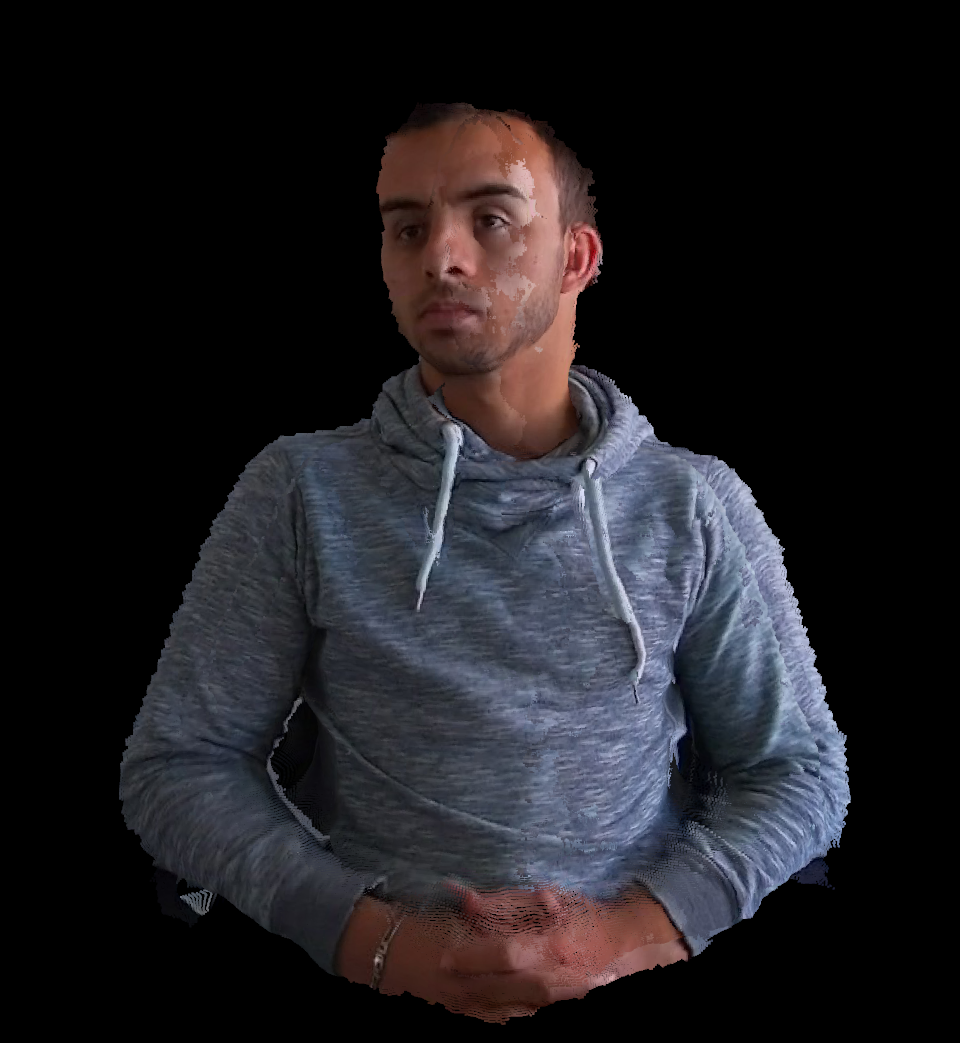
\includegraphics[width=0.35\textwidth]{images/visual_enhancement/colour/raw_colour.png}
    \caption{Merged point cloud. Colour inconsistency clearly visible in the face}
    \label{figure:raw_colour_2}
\end{figure}


\subsubsection{Previous work}

A lot of different approaches have been proposed to correct the colour inconsistency. Nine of these approaches in panoramic images are evaluated in \cite{xu_performance_2010} . These approaches are mainly developed for panoramic imaging. They perform transformations in different colour spaces such as RGB, $Lab$ or YCbCr to take advantage of the properties of that space.

\textbf{Model-based parametric approaches}

Model-based parametric approaches assume a relationship between the colour of the target image and the colour of the source image. \textit{Global modelling} approaches describe this relationship as follow: $I_{s}=M * I_{t}$, where $M$ is a global transformation matrix. It represents the mapping of the three colour channels. Depending on the application and inputs, $M$ can be estimated by various methods. In \cite{gui_yun_tian_colour_2002} a linear and linear with affine model is developed. It uses histogram mapping over the overlap area to estimate $M$. A linear transformation based on statistics of global colour distribution in the uncorrelated $Lab$ colour space is proposed by \cite{reinhard_color_2001}. \textit{Local colour transfer} suggests local mapping. A colour transfer scheme based on probabilistic segmentation and region mapping using Gaussian Mixture Models (GMM) and Expectation-Maximization (EM) is proposed by \cite{yu-wing_tai_local_2005}.


\textbf{Modeless non-parametric approaches}

Some approaches known as non-parametric assume no particular parametric format of the colour mapping function. They mostly use a look-up table to directly record the mapping of the full range of colour/intensity levels. In \cite{xu_performance_2010} some of these approaches are presented.


% L channel holds the brightness and α, β channels
% hold the color information.


\subsubsection{Proposed method}

The idea behind the proposed method is the following: the problem is similar to colour consistency in a panoramic image. The proposed method takes inspiration from \cite{reinhard_color_2001} and \cite{dasari_reference_2016}. The first step consists of finding a Region of Interest (ROI) in a reference/source view and then find the corresponding ROI in the target view. The second step consists of converting the reference ROI and the corresponding ROI of the target image to $Lab$ colour space. Then colour statistics of the source and target image are computed to match them. The final step is called colour parameter optimisation and is processed in the RGB colour space. Figure \ref{figure:colour_correction} shows an overview of the pipeline These three steps will be developed in the following sections:

\begin{enumerate}
\item Extraction of the overlapping region
\item Colour transfer in $Lab$ colour space \cite{reinhard_color_2001}
\item Colour parameter optimisation \cite{dasari_reference_2016}
\end{enumerate}

\begin{figure}[H]
    \centering
    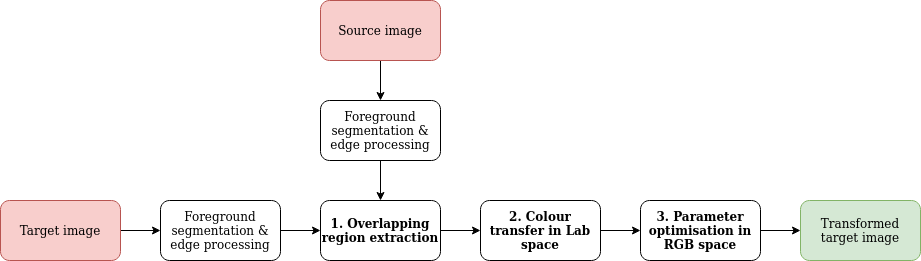
\includegraphics[width=0.99\textwidth]{images/visual_enhancement/colour/colour_correction.png}
    \caption{Proposed pipeline for colour correction. Input: red boxes. Output: green box.}
    \label{figure:colour_correction}
\end{figure}



% The idea is to chose one view as the source image, i.e. the reference image. Then find a region of interest (ROI) in that source that overlaps with a target image. Correct the colour of the target image in the $Lab$ space The proposed pipeline takes inspiration from \cite{dasari_reference_2016}. These are the steps:



\subsubsubsection{Extraction of the overlapping region}
\label{section:Extraction of the overlapping region}

In \cite{dasari_reference_2016}, the extraction of the corresponding ROI between the reference and the target image is based on SIFT feature-matching \cite{lowe_distinctive_2004}. A disadvantage of SIFT is the fact that it can find wrong matching points. Therefore, the performance of the colour correction step is affected. In the proposed approach, SIFT is not used. The corresponding ROI is found thanks to the rigid transformation matrix, presented in section \ref{section:Registration}. The persons are the most important part of a meeting room. They are considered as the ROI of the scene. Here are the steps of finding the corresponding ROI that are illustrated in \ref{figure:overlap}.

\begin{enumerate}
    \item Segment the foreground of the scene, i.e. the humans in the source and target image
    \item Create the point cloud of the 2D source foreground
    \item Transform the source point cloud into the target 3D space thanks to the rigid transformation matrix
    \item Transform the transformed source point cloud into the 2D target pixel space
    \item Find the overlapping region of the source and target foreground in the 2D target space
\end{enumerate}


\begin{figure}[H]
    \centering
    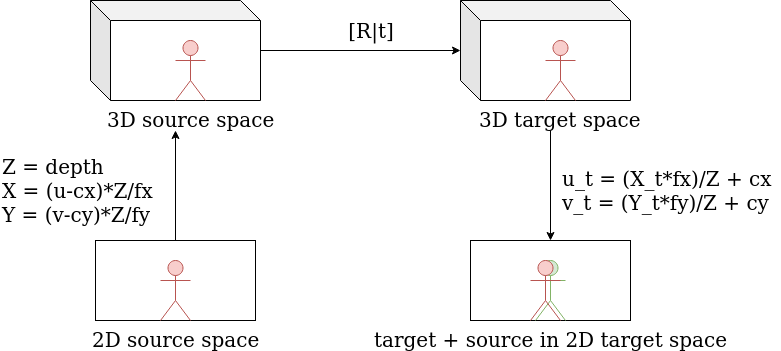
\includegraphics[width=0.65\textwidth]{images/visual_enhancement/colour/overlap.png}
    \caption{Illustration of the process to find the overlapping region. $u, v, u_t, v_t$ are coordinates in pixel. $X, Y, Z, X_t, Y_t$ are coordinates in meter. $fx, fy, cx, cy$ are the intrinsic parameters of the camera. $[R|t]$ is the rigid transformation matrix}
    \label{figure:overlap}
\end{figure}



\subsubsubsection{Colour transfer in $Lab$ colour space}
\label{section:colour tansfer Lab}

The overlapping ROI in both views are converted from RGB to $Lab$ colour space to take advantage of the linearity of that colour space. The uniformity of that colour space is presented in \cite{doi:10.1002/9781119975595.ch3}. $L$ channel represents the brightness and $a$, $b$ channels hold the colour information. The colour transfer is performed using the equation (\ref{equation:colour_transfert}) proposed in \cite{reinhard_color_2001}. It is calculated for each channel independently. The colour transformation is applied on all pixels in a colour channel but $\mu_{s}$, $\sigma_{s}$, $\mu_{t}$ and $\sigma_{t}$ are calculated on the overlapping region only. The results is affected by the quality of the registration.

\begin{equation}
    C_{t}^{\prime}=\mu_{s}+\frac{\sigma_{s}}{\sigma_{t}}\left(C_{t}-\mu_{t}\right)
\label{equation:colour_transfert}
\end{equation}

where:

\begin{itemize}
    \item $C_{t}$ represents a colour channel in the target image
    \item $C_{t}^{\prime}$ represents the transformed colour channel in the target image
    \item $\mu_{s}$ and $\sigma_{s}$ represent mean and standard deviation values of source image
    \item $\mu_{t}$ and $\sigma_{t}$ represent mean and standard deviation values of target image
\end{itemize}



\textbf{Colour parameter optimisation}
\label{section:colour parameter optimisation}

After performing the colour correction in the $Lab$ colour space, the images are converted back in the RGB colour space. Colour parameter optimisation proposed in \cite{dasari_reference_2016} is applied as follow: 

\begin{equation}
    I_{1}=M * I_{2
\label{equation:parameter_optimization}}
\end{equation}

% \begin{equation}
%     \left[\begin{array}{c}
%     {\overrightarrow{I_{1}}} \\
%     {\overrightarrow{I_{2}}} \\
%     {\ldots} \\
%     {\overrightarrow{I_{24}}}
%     \end{array}\right]_{24 \times 3} \times\left[\begin{array}{ccc}
%     {t_{r r}} & {t_{r g}} & {t_{r b}} \\
%     {t_{g r}} & {t_{g g}} & {t_{g b}} \\
%     {r_{b r}} & {t_{b g}} & {t_{b b}}
%     \end{array}\right]_{3 \times 3} \simeq\left[\begin{array}{c}
%     {\overrightarrow{T_{1}}} \\
%     {\overrightarrow{T_{2}}} \\
%     {\cdots} \\
%     {\overrightarrow{T_{24}}}
%     \end{array}\right]_{24 \times 3}
%     \label{equation:rgbTOrgb}
% \end{equation}

\begin{equation}
    M=\left[\begin{array}{ccc}
    {\alpha_{R}} & {0} & {0} \\
    {0} & {\alpha_{G}} & {0} \\
    {0} & {0} & {\alpha_{B}}
\end{array}\right]
\end{equation}

% \begin{equation}
% \begin{aligned}
%     &I_{1}=M * I_{2}\\
%     &M=\left[\begin{array}{ccc}
%     {\alpha_{R}} & {0} & {0} \\
%     {0} & {\alpha_{G}} & {0} \\
%     {0} & {0} & {\alpha_{B}}
% \end{array}\right]
% \end{aligned}
% \label{equation:parameter_optimization}
% \end{equation}

$I_i$ is a 3xN matrix. N is the number of pixels. Each column of $I_i$ represents a pixel with its channel R, G, B.  $\alpha_{R}$, $\alpha_{G}$ and $\alpha_{B}$ are calculated on the overlapped region as follow:

\begin{equation}
    \alpha_{C} = \dfrac{\sum_{i=0}^{n-1} C_{s_{i}}}{\sum_{i=0}^{n-1} C_{t_{i}}}
    \label{equation:param}
\end{equation}

where:

\begin{itemize}
    \item $\alpha_{C}$ represents a channel parameter
    \item $n$ represents the number of pixel in the overlapped region
    \item $C_{t}$ and $C_{s}$ represents a colour channel respectively in the target and source image 
\end{itemize}

\subsubsection{Alternative methods}

Alternative methods have been tested during this project. They are briefly presented in the following sections. They are model-based parametric approaches.

\subsubsubsection{Ensuring Colour Consistency across Multiple Cameras using a colour checkerboard}
\label{section:ensuring_checkerboard}

Using a colour checkerboard to ensure colour consistency is proposed by \cite{ilie_ensuring_2005}. A target like the one in figure \ref{figure:colour_checkerboard} is used to calibrate the colour. It is placed in the middle of the scene and in the field of view of both cameras.

\begin{figure}[H]
    \centering
    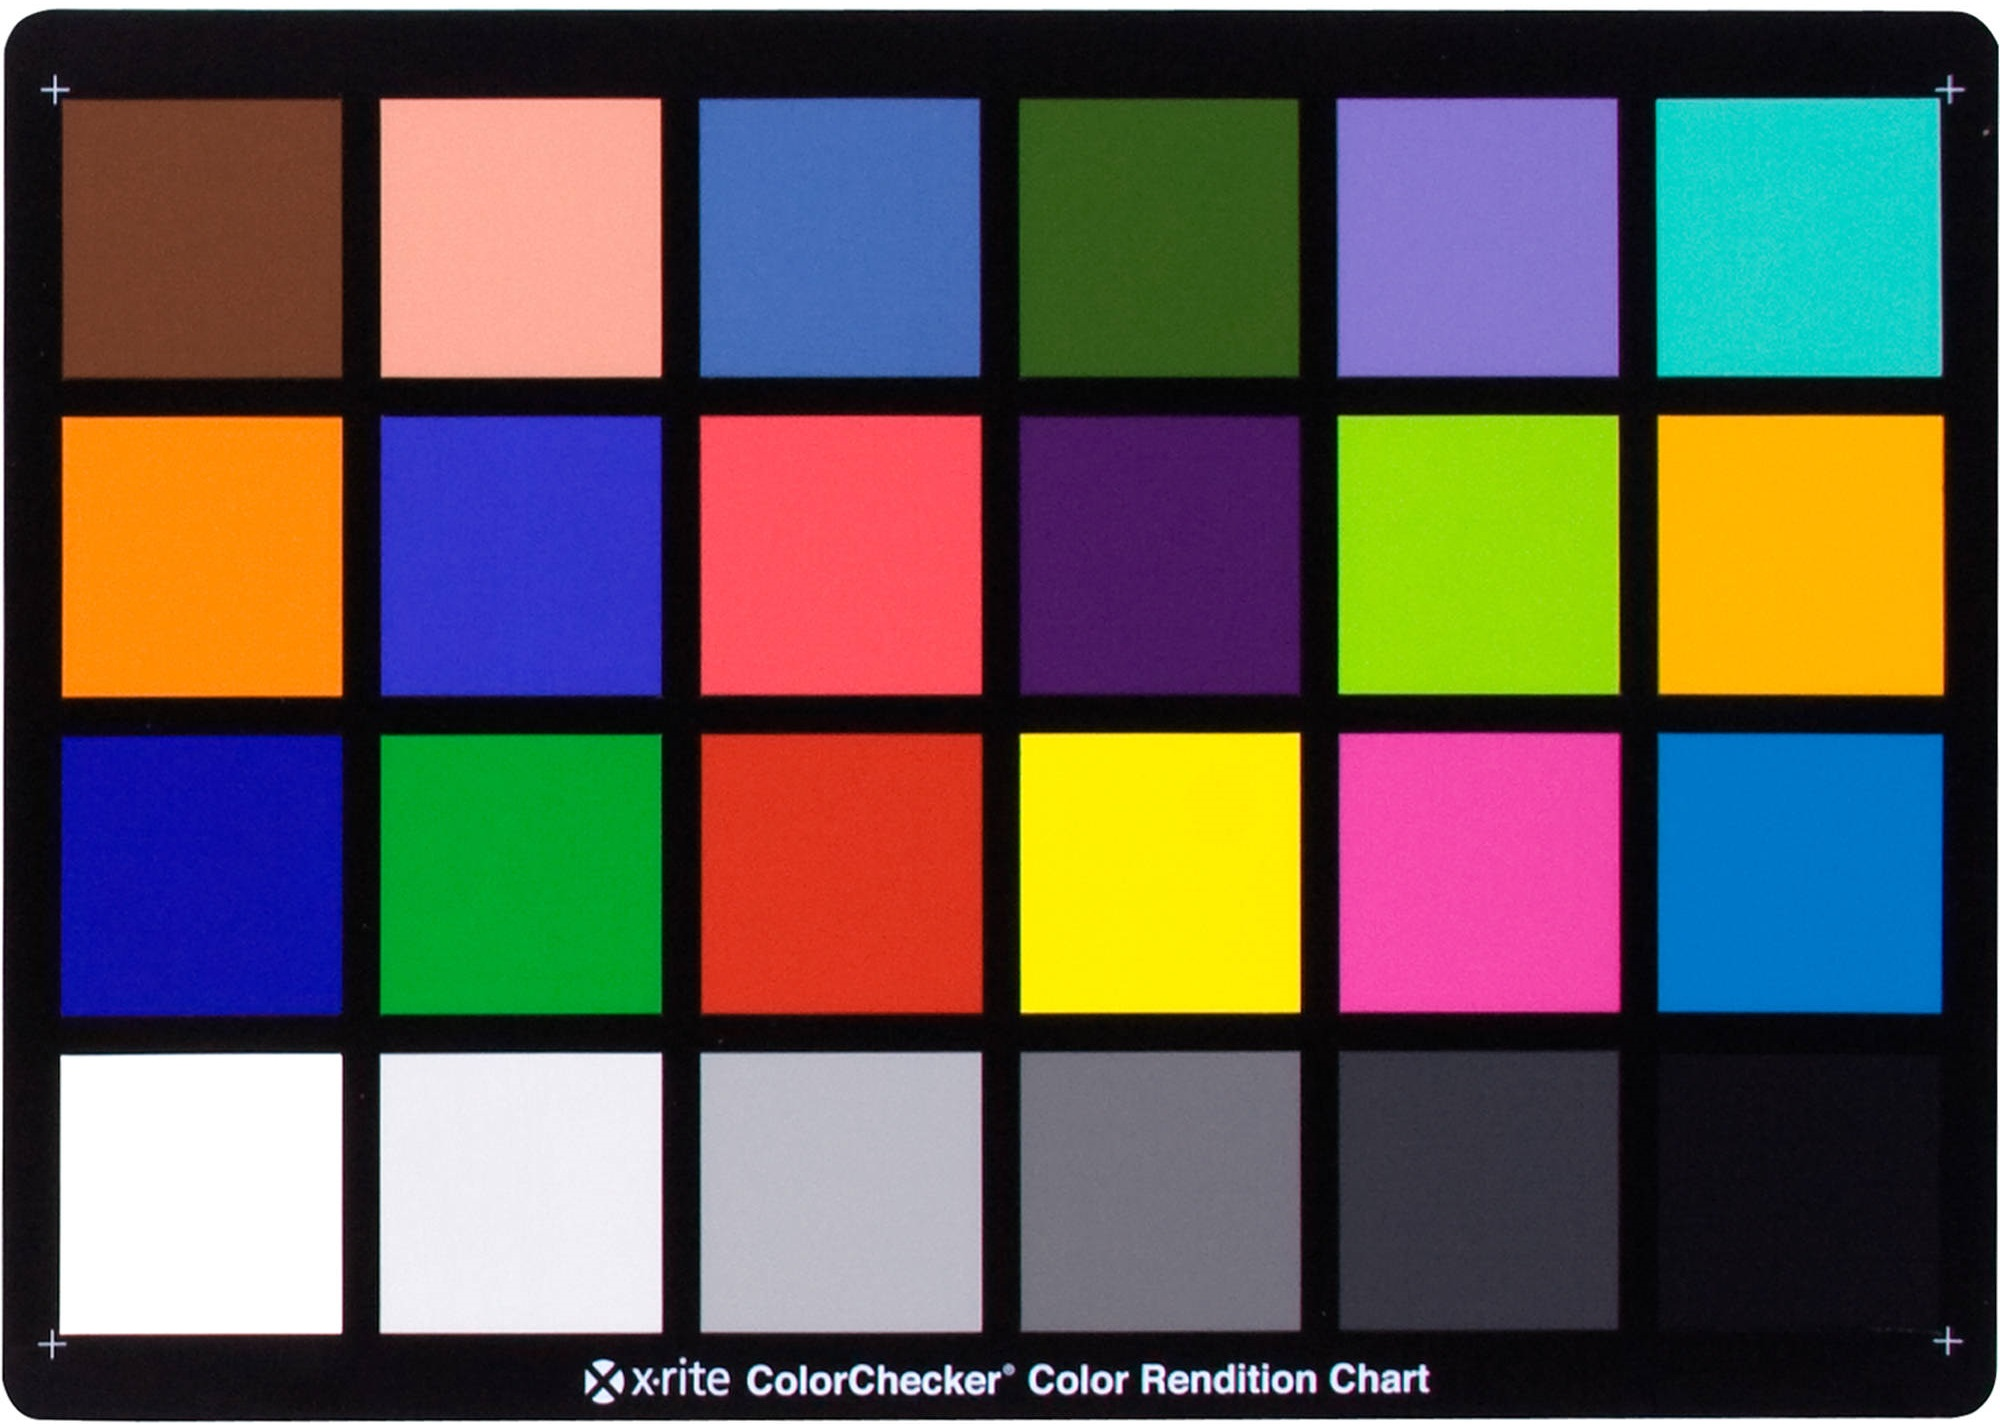
\includegraphics[width=0.40\textwidth]{images/visual_enhancement/colour/colour_checkerboard.jpg}
    \caption{Checkerboard for colour calibration}
    \label{figure:colour_checkerboard}
\end{figure}


The idea is to select one view as the target and the other one as the source. Then, the 24 different colours of the board are detected. Finally, one tries to match them thanks to a transformation. After this transformation is found, it is applied to the whole image. Several methods are proposed in \cite{ilie_ensuring_2005}. They are all applied in the RGB colour space and are briefly presented in the following paragraphs.

\textbf{Linear Least Squares Matching}

The idea is to minimise the equation (\ref{equation:lsm}) in the least square sense. $a$ and $b$ have to be found for each channel independently. Once found the transformation is applied to the entire image. 

\begin{equation}
\sum_{s=1}^{N_s}\left(\vec{I} {c}_{s}-\left(a_{c} \vec{T} {c}_{s}+b_{c}\right)\right)^{2}, c \in\{R, G, B\}
\label{equation:lsm}
\end{equation}

where:

\begin{itemize}
    \item $\vec{I} {c}_{s}$ is the value of a source sample in channel $c$
    \item $\vec{T} {c}_{s}$ is the value of a corresponding target sample in channel $c$
    \item $a_{c}$ \& $b_{c}$ are the parameters to found for each channel $c$
    \item $N_s$ is the number of samples, i.e. 24 in this case, corresponding to the 24 colours of the board
\end{itemize}


\textbf{RGB to RGB Transform}

3x3 RGB to RGB transform is another proposed approach. The purpose is to find a 3x3 matrix that best transforms the 24 colour samples of a source image into the corresponding colour samples of a target image. The matrix is the solution of the matrix system (\ref{equation:rgbTOrgb}). image. The solution is computed thanks to singular value decomposition.

\begin{equation}
    \left[\begin{array}{c}
    {\overrightarrow{I_{1}}} \\
    {\overrightarrow{I_{2}}} \\
    {\ldots} \\
    {\overrightarrow{I_{24}}}
    \end{array}\right]_{24 \times 3} \times\left[\begin{array}{ccc}
    {t_{r r}} & {t_{r g}} & {t_{r b}} \\
    {t_{g r}} & {t_{g g}} & {t_{g b}} \\
    {r_{b r}} & {t_{b g}} & {t_{b b}}
    \end{array}\right]_{3 \times 3} \simeq\left[\begin{array}{c}
    {\overrightarrow{T_{1}}} \\
    {\overrightarrow{T_{2}}} \\
    {\cdots} \\
    {\overrightarrow{T_{24}}}
    \end{array}\right]_{24 \times 3}
    \label{equation:rgbTOrgb}
\end{equation}

where:

\begin{itemize}
    \item $\overrightarrow{I_{s}}=\left[\begin{array}{lll}{I r_{s}} & {I g_{s}} & {I b_{s}}\end{array}\right]$ is the colour for source sample $s$
    \item $\vec{T}_{s}=\left[Tr_{s}  T g_{s}  T b_{s}\right]$ is the colour for target sample $s$
    \item $t_{x y}$ is the term that specifies how much the input from
colour channel x contributes to the output of colour channel y
\end{itemize}



\textbf{General Polynomial Transform}

RGB to RGB matrix transform doesn't have a translation component and doesn't compensate for non-linearity. Therefore, general polynomial transform is proposed to take into account these observations. The proposed general formula is the following one:

\begin{equation}
    \sum_{k=1}^{D}\left(t_{r c_{k}} I r_{s}^{k}+t_{g c_{k}} I g_{s}^{k}+t_{b c_{k}} I b_{s}^{k}\right)+t_{c 0} \simeq T c_{s}
\label{equation:general_polynomial_transform}
\end{equation}

where:

\begin{itemize}
    \item $D$ is the degree of the polynomial approximation
    \item $I r_{s}^{k}, I g_{s}^{k}$ \& $I b_{s}^{k}$ are the red, green and blue values for source image sample $s$, raised to power $k$
    \item $T c_{s}$ is the value for colour channel $c$ of target image sample $s$
    \item $t_{r c_{k}}$ is the polynomial coefficient of the $k^{th}$ order term that indicates how much the input from colour channel $x \in\ {r, g, b}$ contributes to the output of colour channel $c$
    \item $t_{c 0}$ is a term that translates the output of channel $c$
\end{itemize}


\subsubsubsection{Colour Correction Using 3D Multiview Geometry}

An approach based on corresponding matching points is proposed by \cite{eschbach_color_2015}. Polynomial regression is chosen to find the relation between a reference view and the other views. Equations (\ref{equation:pol_reg_2015}) and (\ref{equation:pol_reg_2015_theta}) develop the computation for a channel. The polynomial regression is calculated for each channel independently. Once the translation matrices are found, they are applied to the whole image.

% \begin{equation}
% \mathbf{X}_{\mathrm{r}}=\left[\begin{array}{cccccc}
% {1} & {r_{\mathrm{s} 1}} & {r_{\mathrm{s} 1}^{2}} & {r_{\mathrm{s} 1}^{3}} & {r_{\mathrm{s} 1}^{4}} & {r_{\mathrm{s} 1}^{5}} \\
% {1} & {r_{\mathrm{s} 2}} & {r_{\mathrm{s} 2}^{2}} & {r_{\mathrm{s} 2}^{3}} & {r_{\mathrm{s} 2}^{4}} & {r_{\mathrm{s} 2}^{5}} \\
% {} & {} & {} & {\vdots} & {} \\
% {1} & {r_{\mathrm{sn}}} & {r_{\mathrm{sn}}^{2}} & {r_{\mathrm{sn}}^{3}} & {r_{\mathrm{sn}}^{4}}
% \end{array}\right], \mathbf{Y}_{\mathrm{r}}=\left[\begin{array}{c}
% {r_{11}} \\
% {r_{12}} \\
% {\vdots} \\
% {r_{m}}
% \end{array}\right]
% \label{equation:pol_reg_2015}
% \end{equation}

% \begin{equation}
% \boldsymbol{\theta}_{\mathrm{r}}=\left(\mathbf{X}_{\mathrm{r}}^{\mathrm{T}} \mathbf{X}_{\mathrm{r}}\right)^{-1} \mathbf{X}_{\mathrm{r}}^{\mathrm{T}} \mathbf{Y}_{\mathrm{r}}
% \label{equation:pol_reg_2015_theta}
% \end{equation}


\begin{equation}
\mathbf{X}_{\mathrm{c}}=\left[\begin{array}{cccccc}
{1} & {c_{\mathrm{s} 1}} & {c_{\mathrm{s} 1}^{2}} & {c_{\mathrm{s} 1}^{3}} & {c_{\mathrm{s} 1}^{4}} & {c_{\mathrm{s} 1}^{5}} \\
{1} & {c_{\mathrm{s} 2}} & {c_{\mathrm{s} 2}^{2}} & {c_{\mathrm{s} 2}^{3}} & {c_{\mathrm{s} 2}^{4}} & {c_{\mathrm{s} 2}^{5}} \\
{} & {} & {} & {\vdots} & {} \\
{1} & {c_{\mathrm{sn}}} & {c_{\mathrm{sn}}^{2}} & {c_{\mathrm{sn}}^{3}} & {c_{\mathrm{sn}}^{4}} & {c_{\mathrm{sn}}^{5}}
\end{array}\right], \mathbf{Y}_{\mathrm{c}}=\left[\begin{array}{c}
{c_\mathrm{t1}} \\
{c_\mathrm{t2}} \\
{\vdots} \\
{c_\mathrm{tn}}
\end{array}\right]
\label{equation:pol_reg_2015}
\end{equation}

\begin{equation}
\boldsymbol{\theta}_{\mathrm{c}}=\left(\mathbf{X}_{\mathrm{c}}^{\mathrm{T}} \mathbf{X}_{\mathrm{c}}\right)^{-1} \mathbf{X}_{\mathrm{c}}^{\mathrm{T}} \mathbf{Y}_{\mathrm{c}}
\label{equation:pol_reg_2015_theta}
\end{equation}

where:

\begin{itemize}
\item $c_\mathrm{sn}$ represents a value for a pixel in a source viewpoint in a channel. $c \in\{R, G, B\}$
\item $c_\mathrm{tn}$ represents a value for a pixel in the target viewpoint in a channel. $c \in\{R, G, B\}$
\item $\theta_{\mathrm{c}}$ is the translation matrix of a channel. $c \in\{R, G, B\}$
\end{itemize}


\subsubsection{Result proposed method}

% The performance of the algorithms are evaluated on a selected frame. In the video stream application, the found transformation is applied on all frames. The fact that the inconsistency in the colour is similar within an experiment is a made assumption.

% \textbf{Proposed method}

The performance of the proposed method is evaluated on a selected frame. This selected frame is first processed through the edge processing step to avoid wrong colour part in the overlapping region. Figure \ref{figure:processed_raw_colour} shows the initial merged point cloud created from both views after applying edge processing.

\begin{figure}[H]
    \centering
    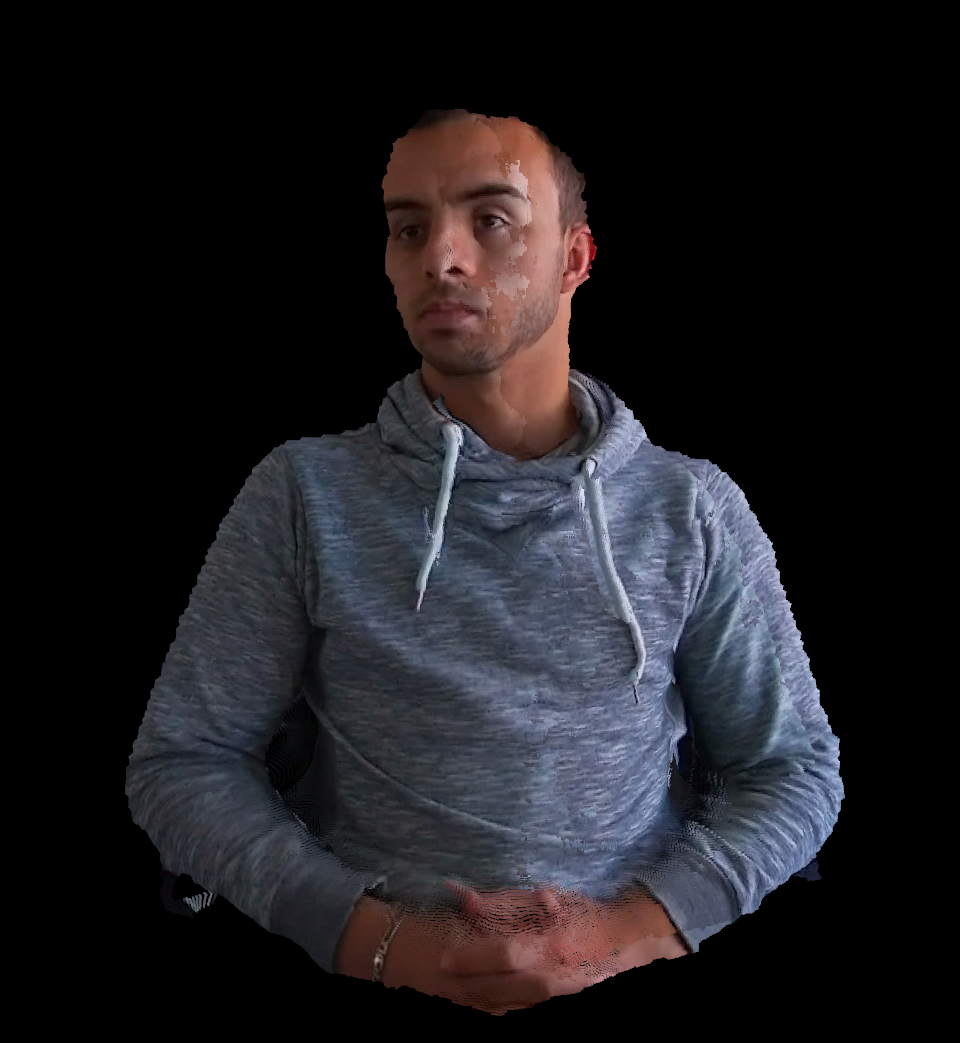
\includegraphics[width=0.3\textwidth]{images/visual_enhancement/colour/processed_raw_colour.png}
    \caption{Merged point cloud. Colour inconsistency after edge processing}
    \label{figure:processed_raw_colour}
\end{figure}

\subsubsubsection{Extraction of the overlapping region}

Presented in section \ref{section:Extraction of the overlapping region}, the algorithm to extract the overlapping region is applied. It founds the ROI in both views as shown in figure \ref{figure:overlap_200}.

% \begin{figure}[H]
% \centering
%   \begin{subfigure}[b]{0.35 \textwidth}
%     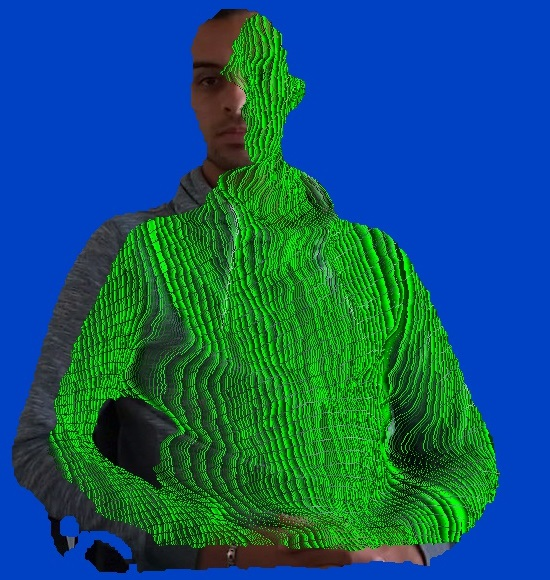
\includegraphics[width=\textwidth]{images/visual_enhancement/colour/sub_overlap_200.jpg}
%     \caption{2D RGB view from camera 1}
%     \label{figure:sub_overlap_200}
%   \end{subfigure}
%   \hfill
%   \begin{subfigure}[b]{0.35 \textwidth}
%     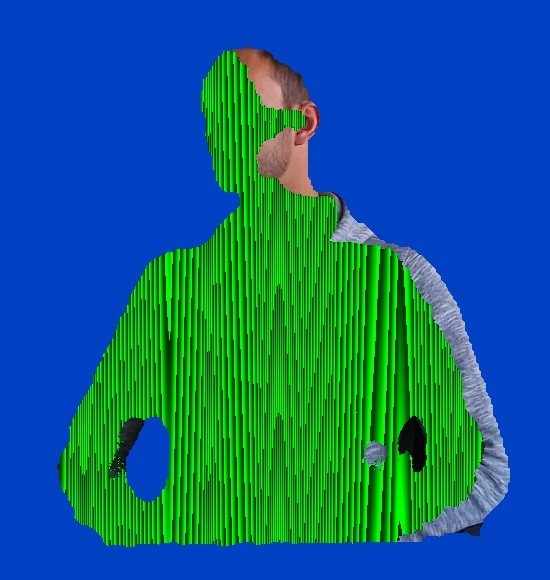
\includegraphics[width=\textwidth]{images/visual_enhancement/colour/master_overlap_200.jpg}
%     \caption{2D RGB view from camera 2}
%     \label{figure:master_overlap_200}
%   \end{subfigure}
%   \caption{Same scene views from two cameras. The greenish region is the overlapping part of the scene.}
%   \label{figure:overlap_200}
% \end{figure}



\begin{figure}[H]

\begin{multicols}{2}
        \begin{subfigure}{\linewidth}
               \centering
                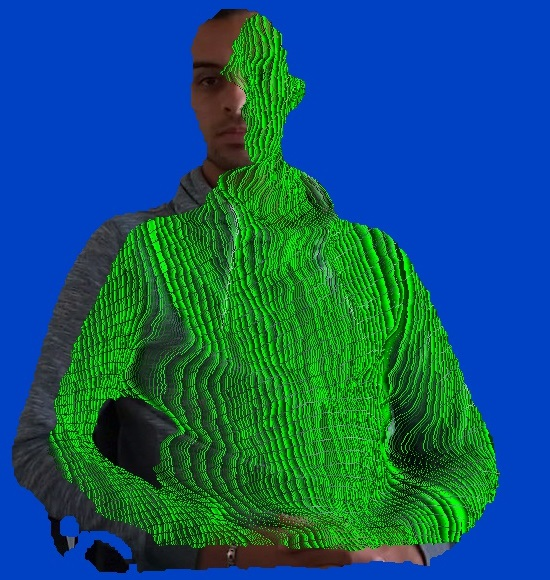
\includegraphics[width=.75\linewidth]{images/visual_enhancement/colour/sub_overlap_200.jpg}
               \caption{2D RGB view from camera 1}\label{figure:sub_overlap_200}
        \end{subfigure}
        
        
        \begin{subfigure}{\linewidth}
               \centering
             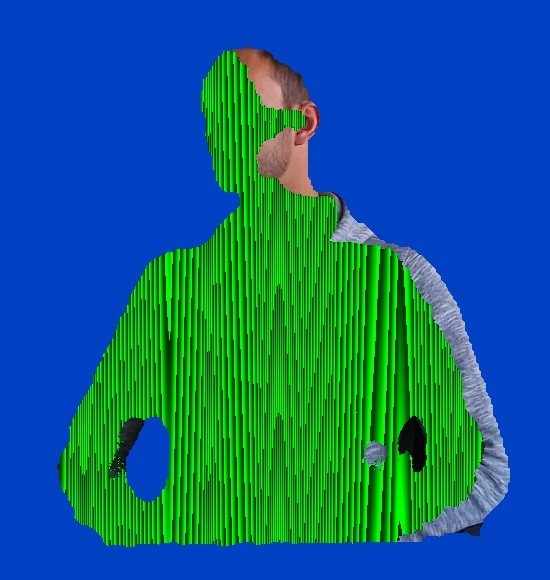
\includegraphics[width=.75\linewidth]{images/visual_enhancement/colour/master_overlap_200.jpg}
               \caption{2D RGB view from camera 2}\label{figure:master_overlap_200}
        \end{subfigure}
\end{multicols}\vspace{-10pt}
\caption{Same scene views from two cameras. The greenish region is the overlapping part of the scene.}
\label{figure:overlap_200}

\end{figure}


Figure \ref{figure:overlap_region} shows the created point cloud from the two views. The greenish region is the one that overlaps in both views. The colour information of that region is used for the next step, i.e. colour transfer in $Lab$ colour space.

\begin{figure}[H]
    \centering
    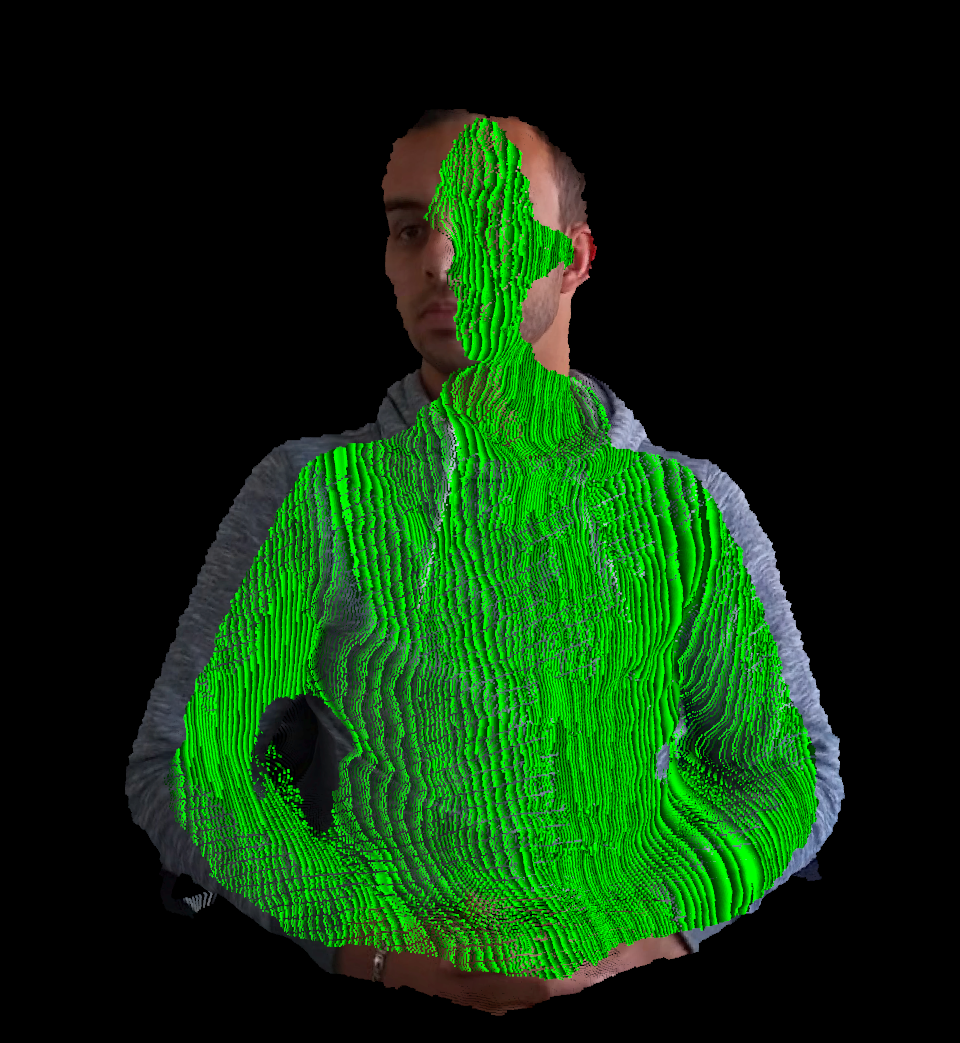
\includegraphics[width=0.35\textwidth]{images/visual_enhancement/colour/overlap_region.png}
    \caption{Merged point cloud. Overlapping region}
    \label{figure:overlap_region}
\end{figure}

\subsubsubsection{Colour tansfer Lab}

The overlapping region is transformed in $Lab$ colour space. The statistics of these ROI are calculated for both views. Table \ref{tab:stat_overlap} presents the found value. The last row contains the result after applying the transformation of the equation (\ref{equation:colour_transfert}).

\begin{table}[H]
\centering
\begin{tabular}{c|c|c|c||c|c|c}
 & \textbf{Mean $L$} & \textbf{Mean $a$} & \textbf{Mean $b$} & \textbf{Std $L$} & \textbf{Std $a$} & \textbf{std $b$} \\ \hline
\textbf{\begin{tabular}[c]{@{}c@{}}Source\\ ROI\end{tabular}} & 85.35 & 132.65 & 120.80 & 36.88 & 6.24 & 10.18 \\ \hline
\textbf{\begin{tabular}[c]{@{}c@{}}Target\\ ROI\end{tabular}} & 91.07 & 131.07 & 120.59 & 45.67 & 5.85 & 9.02 \\ \hline \hline
\textbf{\begin{tabular}[c]{@{}c@{}}Transformed target\\ ROI\end{tabular}} & 84.84 & 132.21 & 120.26 & 36.89 & 6.19 & 10.20
\end{tabular}
\caption{Statistics of the overlapping region. They are calculated over the 113470 pixels of the overlapping region.}
\label{tab:stat_overlap}
\end{table}

Figure \ref{figure:overlap_region_lab} shows the result after applying the colour transfer equation (\ref{equation:colour_transfert}) in the $Lab$ colour space and then transformed back in the RGB colour space.

\begin{figure}[H]
    \centering
    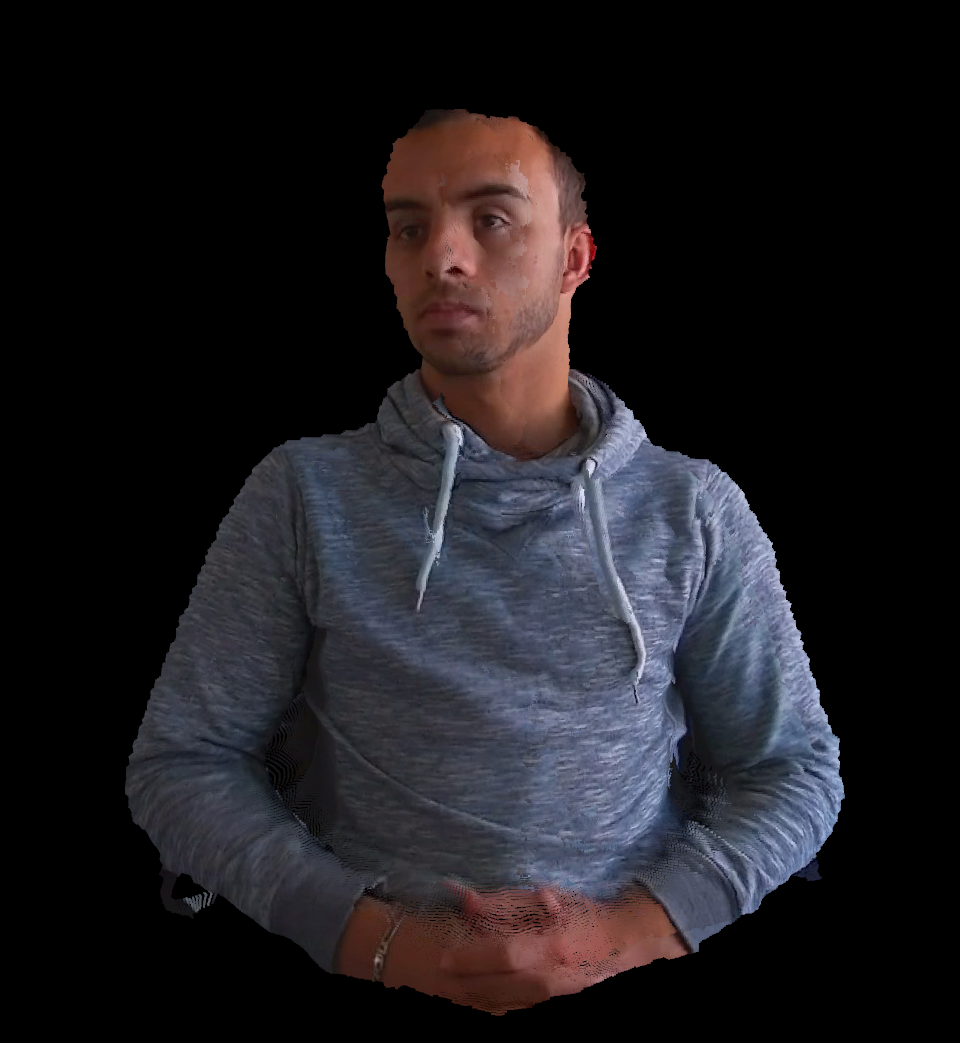
\includegraphics[width=0.35\textwidth]{images/visual_enhancement/colour/overlap_region_lab.png}
    \caption{Merged point cloud. Colour correction result after colour transfer in $Lab$ colour space}
    \label{figure:overlap_region_lab}
\end{figure}

\subsubsubsection{Colour parameter optimisation}

The overlapping regions are transformed back into the RGB colour space. Equation (\ref{equation:param}) is then used to calculate the coefficient between the transformed target ROI and the source ROI. Table \ref{tab:parameters} shows the found coefficients.

\begin{table}[H]
\centering
    \begin{tabular}{c|c|c}
    \textbf{$\mathbf{\alpha_{R}}$} & \textbf{$\mathbf{\alpha_{G}}$} & \textbf{$\mathbf{\alpha_{B}}$} \\ \hline
    0.93 & 0.93 & 0.96
    \end{tabular}
\caption{Found parameters}
\label{tab:parameters}
\end{table}



Each channel of the transformed targeted image is multiplied by the found parameters. Figure \ref{figure:param_opt_lab} shows the result after this colour parameter optimisation step. 

\begin{figure}[H]
    \centering
    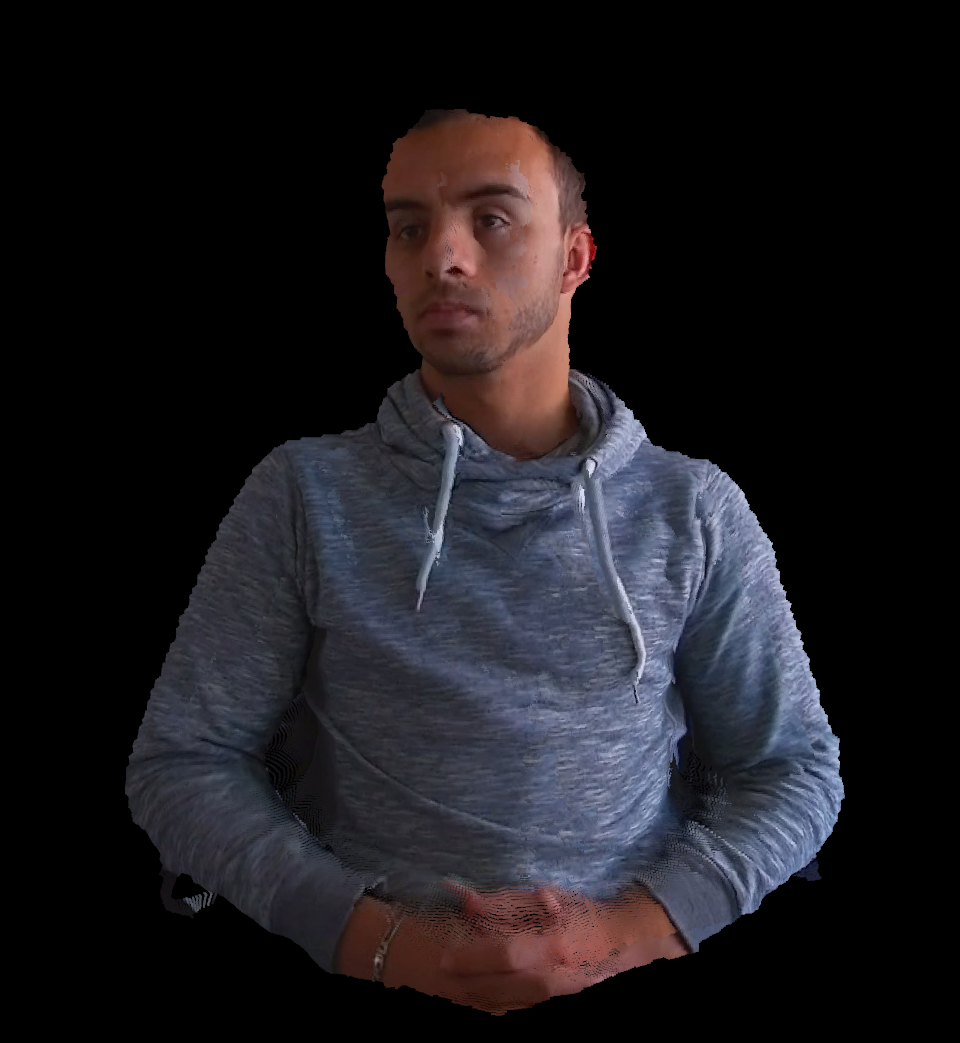
\includegraphics[width=0.35\textwidth]{images/visual_enhancement/colour/param_opt_lab.png}
    \caption{Merged point cloud. Colour correction result after colour parameter optimisation step}
    \label{figure:param_opt_lab}
\end{figure}

\subsubsection{General results of the proposed method}

Table \ref{tab:mse_color} shows the performance of the colour correction algorithms. Mean square error (MSE) metric is chosen to evaluate these algorithms. This evaluation process is the one proposed by the paper \cite{dasari_reference_2016}. The error is calculated for each channel independently.

\begin{table}[H]
\begin{tabular}{c|c|c|c}
\textbf{} & \textbf{MSE R} & \textbf{MSE G} & \textbf{MSE B} \\ \hline
\textbf{No colour correction} & 87.31 & 88.18 & 89.81 \\ \hline
\textbf{$Lab$ colour space correction} & 79.98 & 80.09 & 82.55 \\ \hline
\textbf{$Lab$ colour space correction + parameter optimisation} & 72.79 & 74.69 & 77.72
\end{tabular}
\caption{Performance colour correction pixelwise}
\label{tab:mse_color}
\end{table}


\begin{figure}[H]
\centering
  \begin{subfigure}[b]{0.32 \textwidth}
    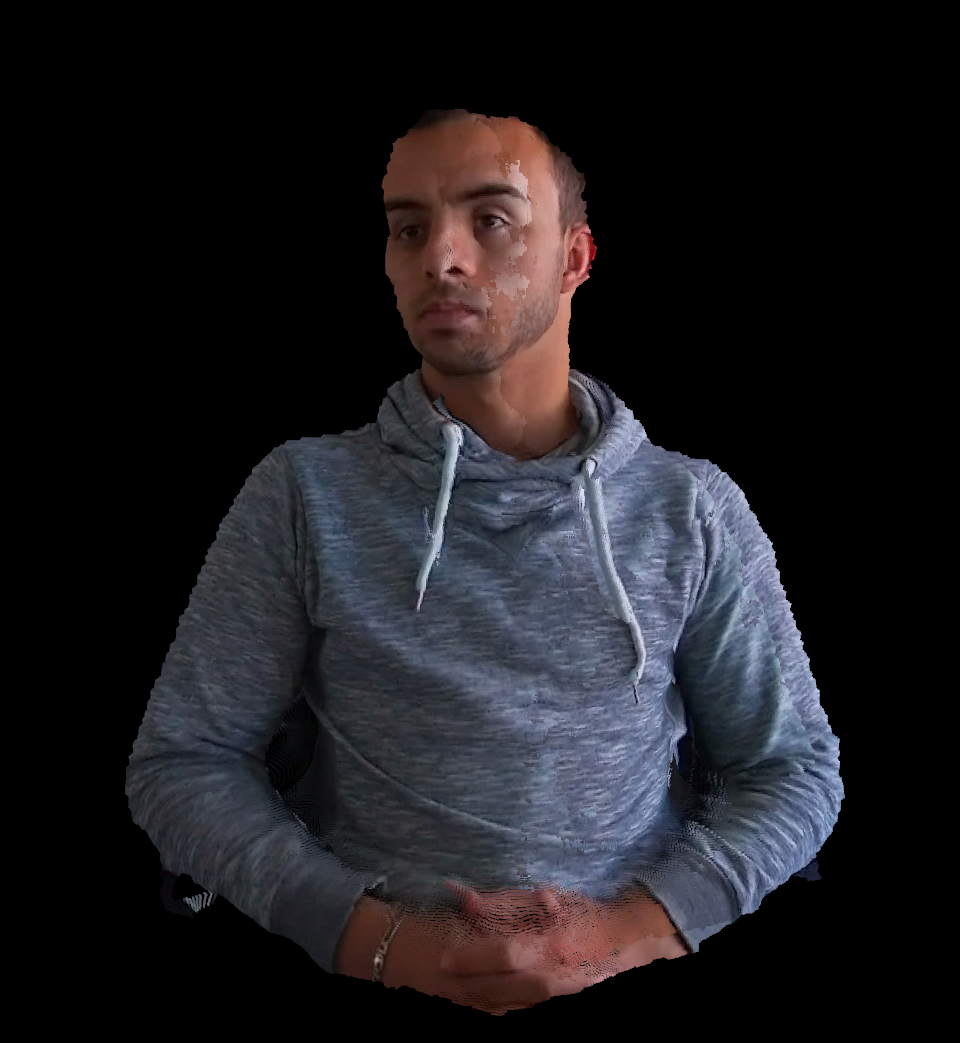
\includegraphics[width=\textwidth]{images/visual_enhancement/colour/processed_raw_colour.png}
    \caption{Raw merged point cloud}
    \label{figure:processed_raw_colour_2}
  \end{subfigure}
  \hfill
  \begin{subfigure}[b]{0.32 \textwidth}
    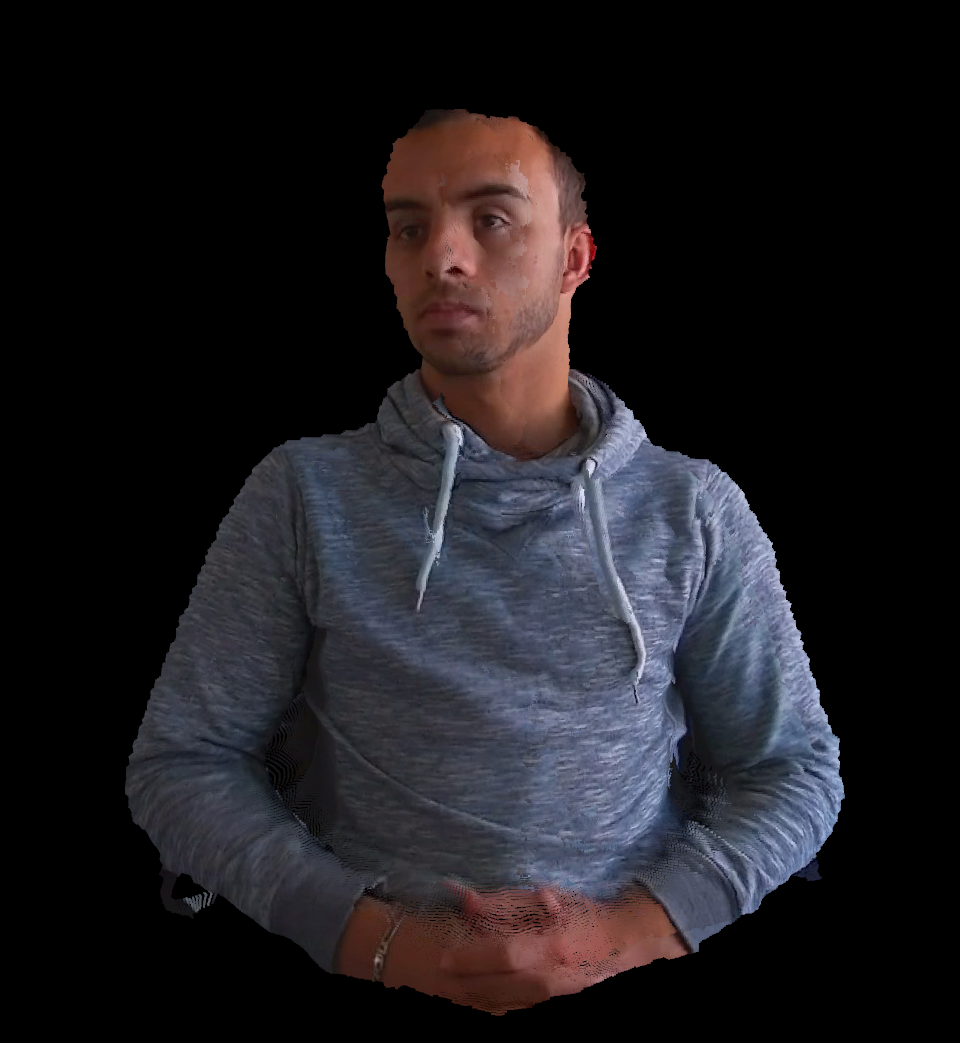
\includegraphics[width=\textwidth]{images/visual_enhancement/colour/overlap_region_lab.png}
    \caption{Colour transfer in Lab space}
    \label{figure:overlap_region_lab_2}
  \end{subfigure}
  \hfill
  \begin{subfigure}[b]{0.32 \textwidth}
    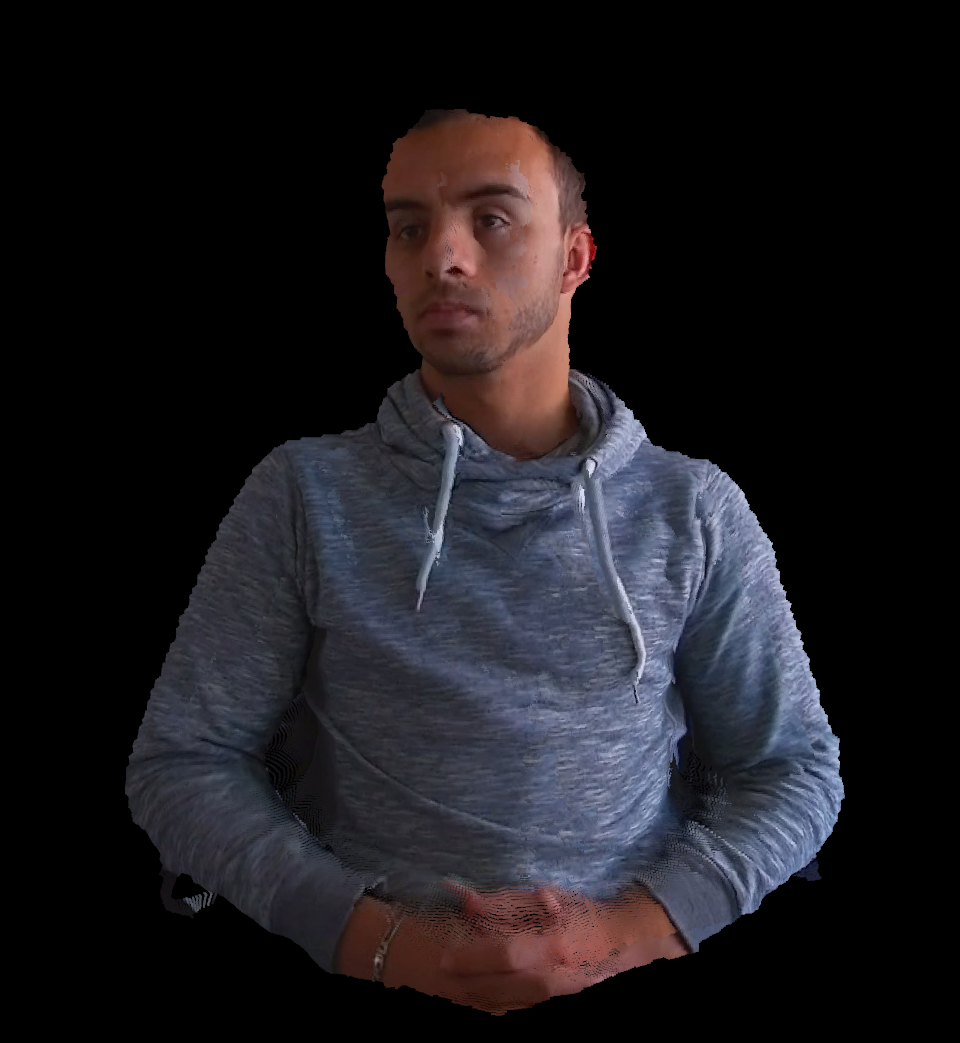
\includegraphics[width=\textwidth]{images/visual_enhancement/colour/param_opt_lab.png}
    \caption{Colour parameter optimisation}
    \label{figure:param_opt_lab_2}
  \end{subfigure}
  \caption{Comparison of the merged point cloud after each step of the colour correction process.}
  \label{figure:summary_colour_correction}
\end{figure}


\subsubsection{ Result alternative methods}

\subsubsubsection{Ensuring Colour Consistency across Multiple Cameras using a colour checker-board}
\label{section:exp_ens_checkerboard}
\textbf{Set-up description}

Some approaches proposes in \cite{ilie_ensuring_2005} and presented in section \ref{section:ensuring_checkerboard} were applied in this experiment. A homemade colour checkerboard was created, see figure \ref{figure:charuco24_color}. It takes advantage of the ArUco pattern for the detection. The algorithm used in section \ref{section:charuco_board_corners} was reused to detect the corners of the colour squares.

\begin{figure}[H]
    \centering
    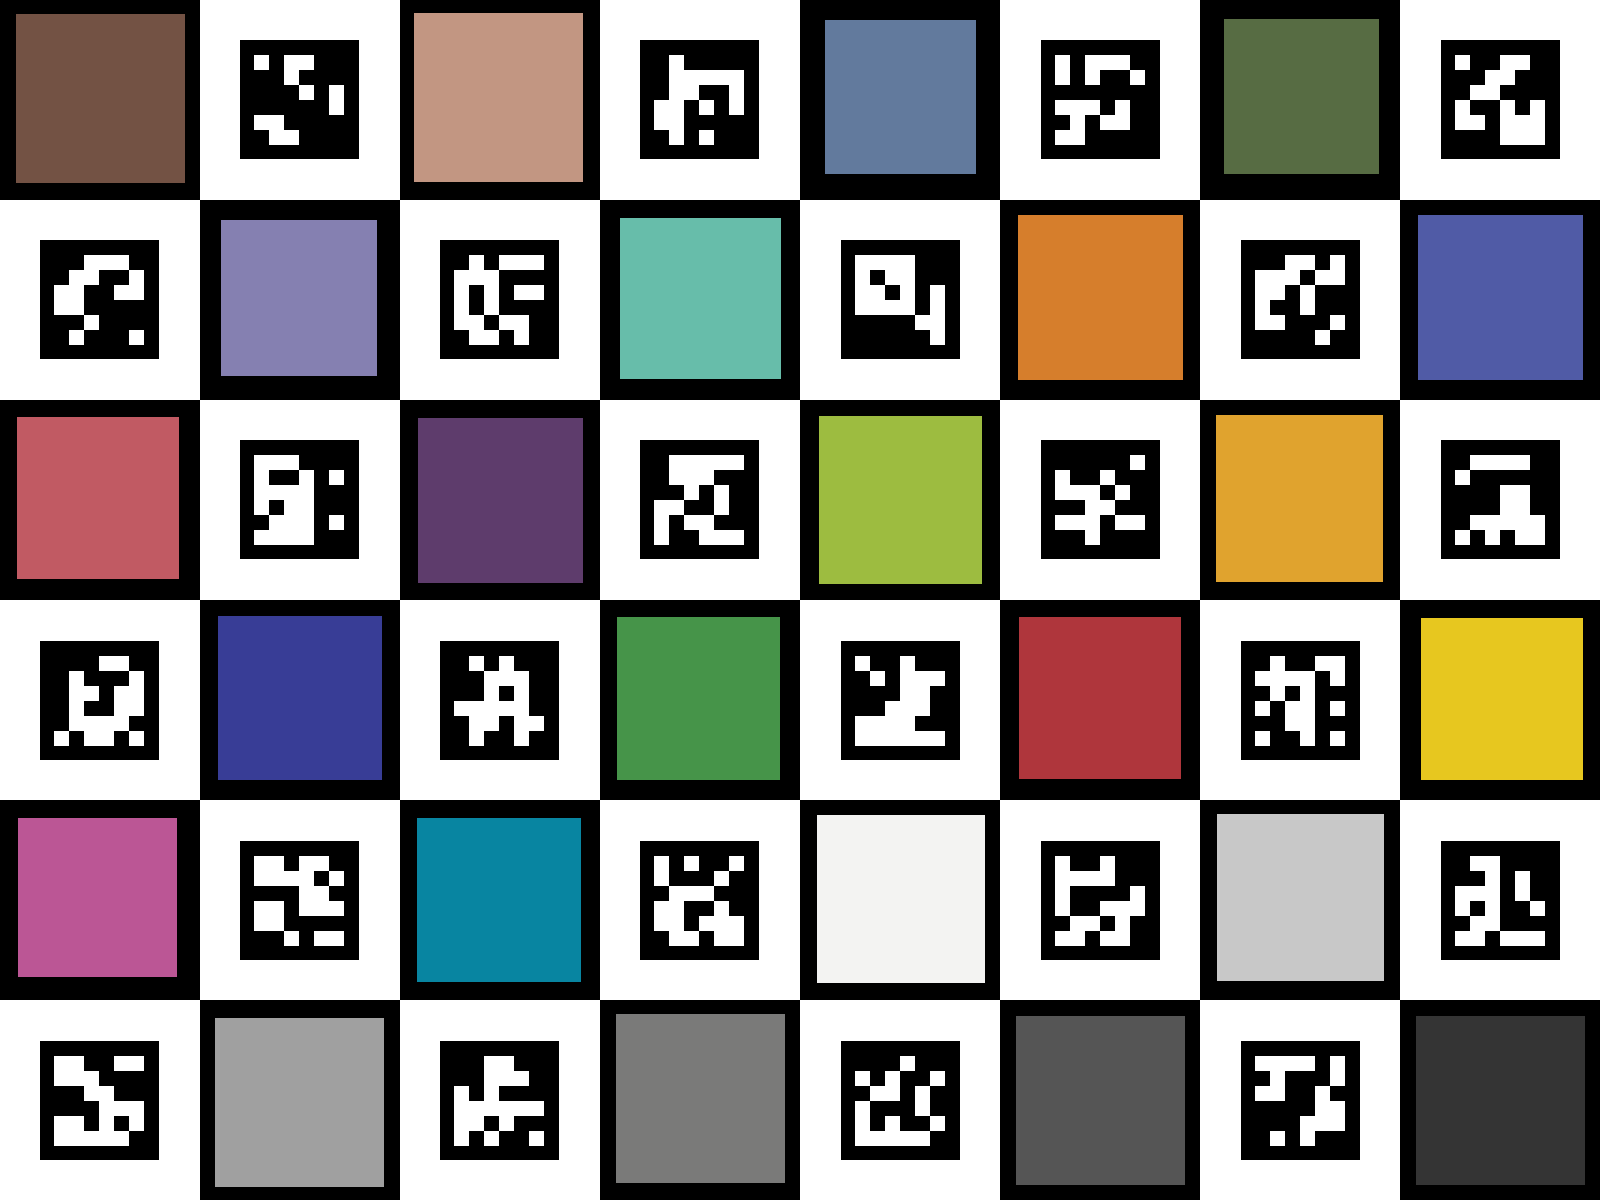
\includegraphics[width=0.40\textwidth]{images/visual_enhancement/colour/charuco24_color.png}
    \caption{Home made colour checkerboard}
    \label{figure:charuco24_color}
\end{figure}

The board was placed in the middle of the scene, see figure \ref{figure:checkerboard_00050}. The average value of the colour was calculated for each view in order to create two datasets of 24 values, i.e. one value per colour, and 3 columns corresponding to the channels R, G and B.
These 2 datasets are used for testing the different approaches proposed in \cite{ilie_ensuring_2005}.

\begin{figure}[H]
\centering
  \begin{subfigure}[b]{0.48 \textwidth}
    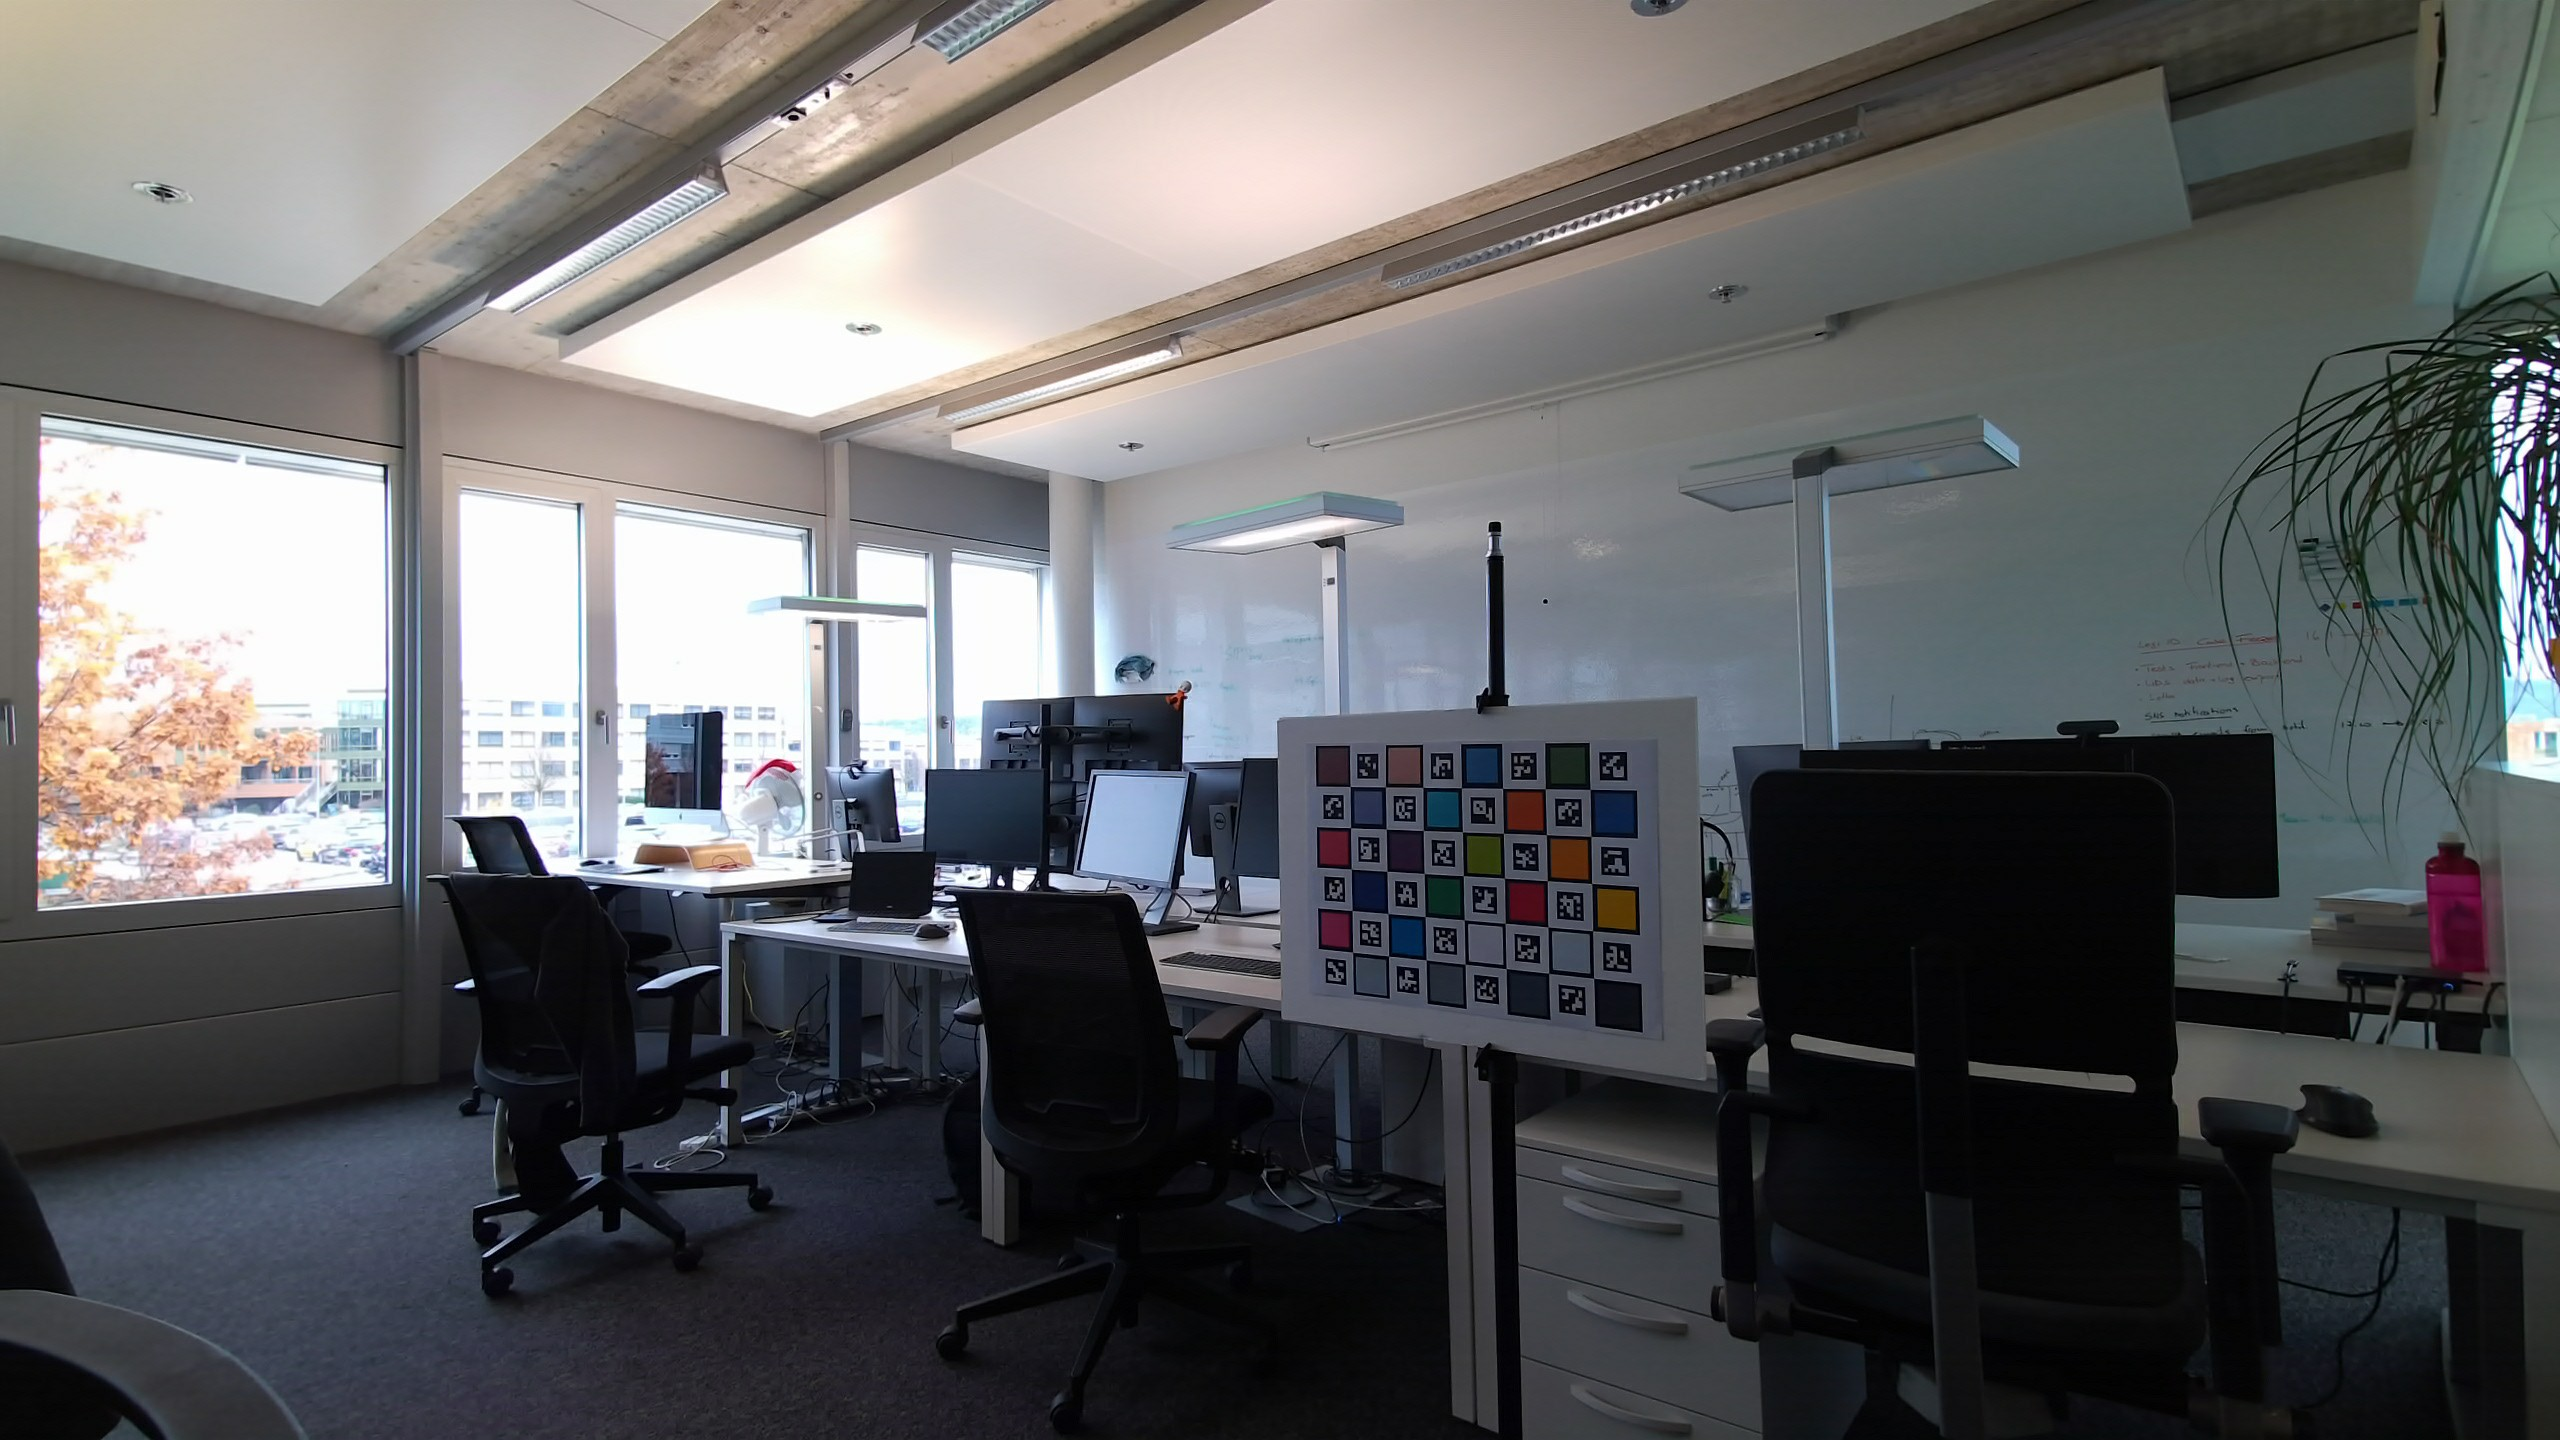
\includegraphics[width=\textwidth]{images/visual_enhancement/colour/master_checkerboard_00050.jpg}
    \caption{View from camera 1}
    \label{figure:master_checkerboard_00050}
  \end{subfigure}
  \hfill
  \begin{subfigure}[b]{0.48 \textwidth}
    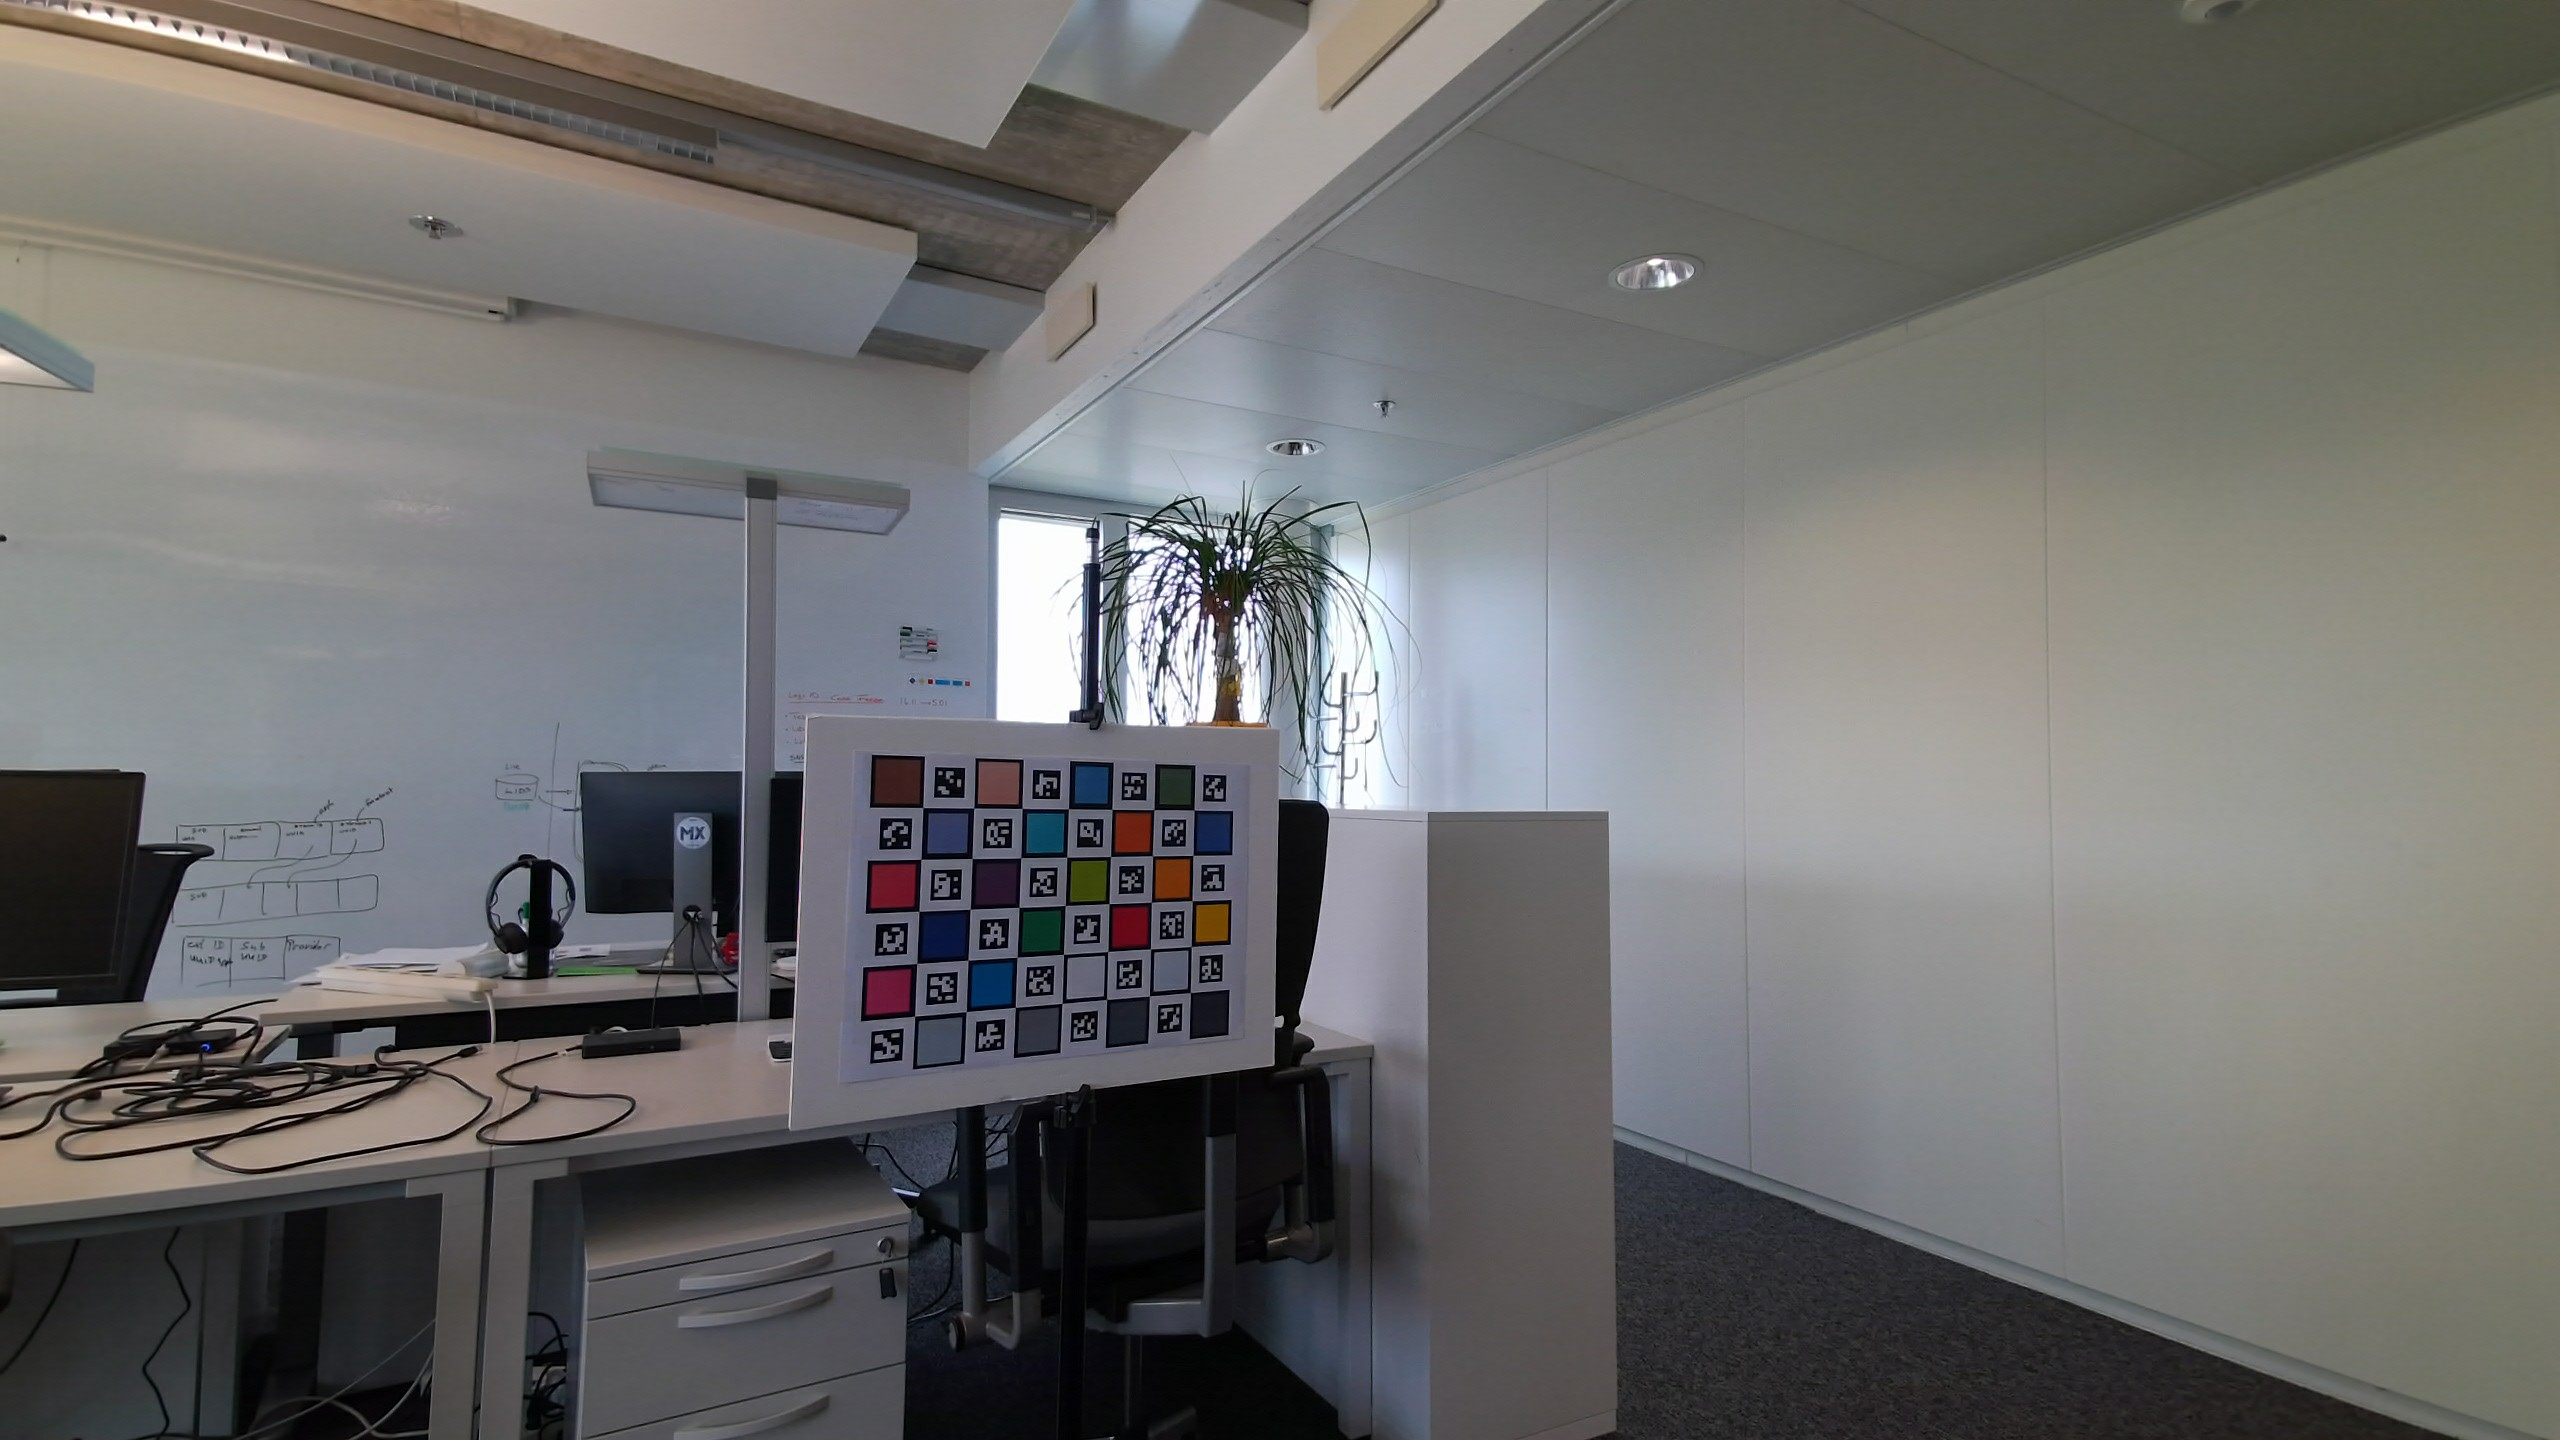
\includegraphics[width=\textwidth]{images/visual_enhancement/colour/sub_checkerboard_00050.jpg}
    \caption{View from camera 2}
    \label{figure:sub_checkerboard_00050}
  \end{subfigure}
  \caption{Colour checkerboard in the middle of the scene. The view \ref{figure:sub_checkerboard_00050} looks brighter than the view \ref{figure:master_checkerboard_00050} }
  \label{figure:checkerboard_00050}
\end{figure}

The following algorithms find colour transformations to modify \ref{figure:sub_checkerboard_00050} in order to match the colour of \ref{figure:master_checkerboard_00050}. The 24 colours of image \ref{figure:master_checkerboard_00050} are defined as reference.

\textbf{Linear Least Squares Matching}

The parameters for each channel were found thanks to equation \ref{equation:lsm}. Despite an amelioration in the colour of the board, the transformation doesn't improve much the rendering, see figure \ref{figure:sub_poly_1_2015}.

\begin{figure}[H]
    \centering
    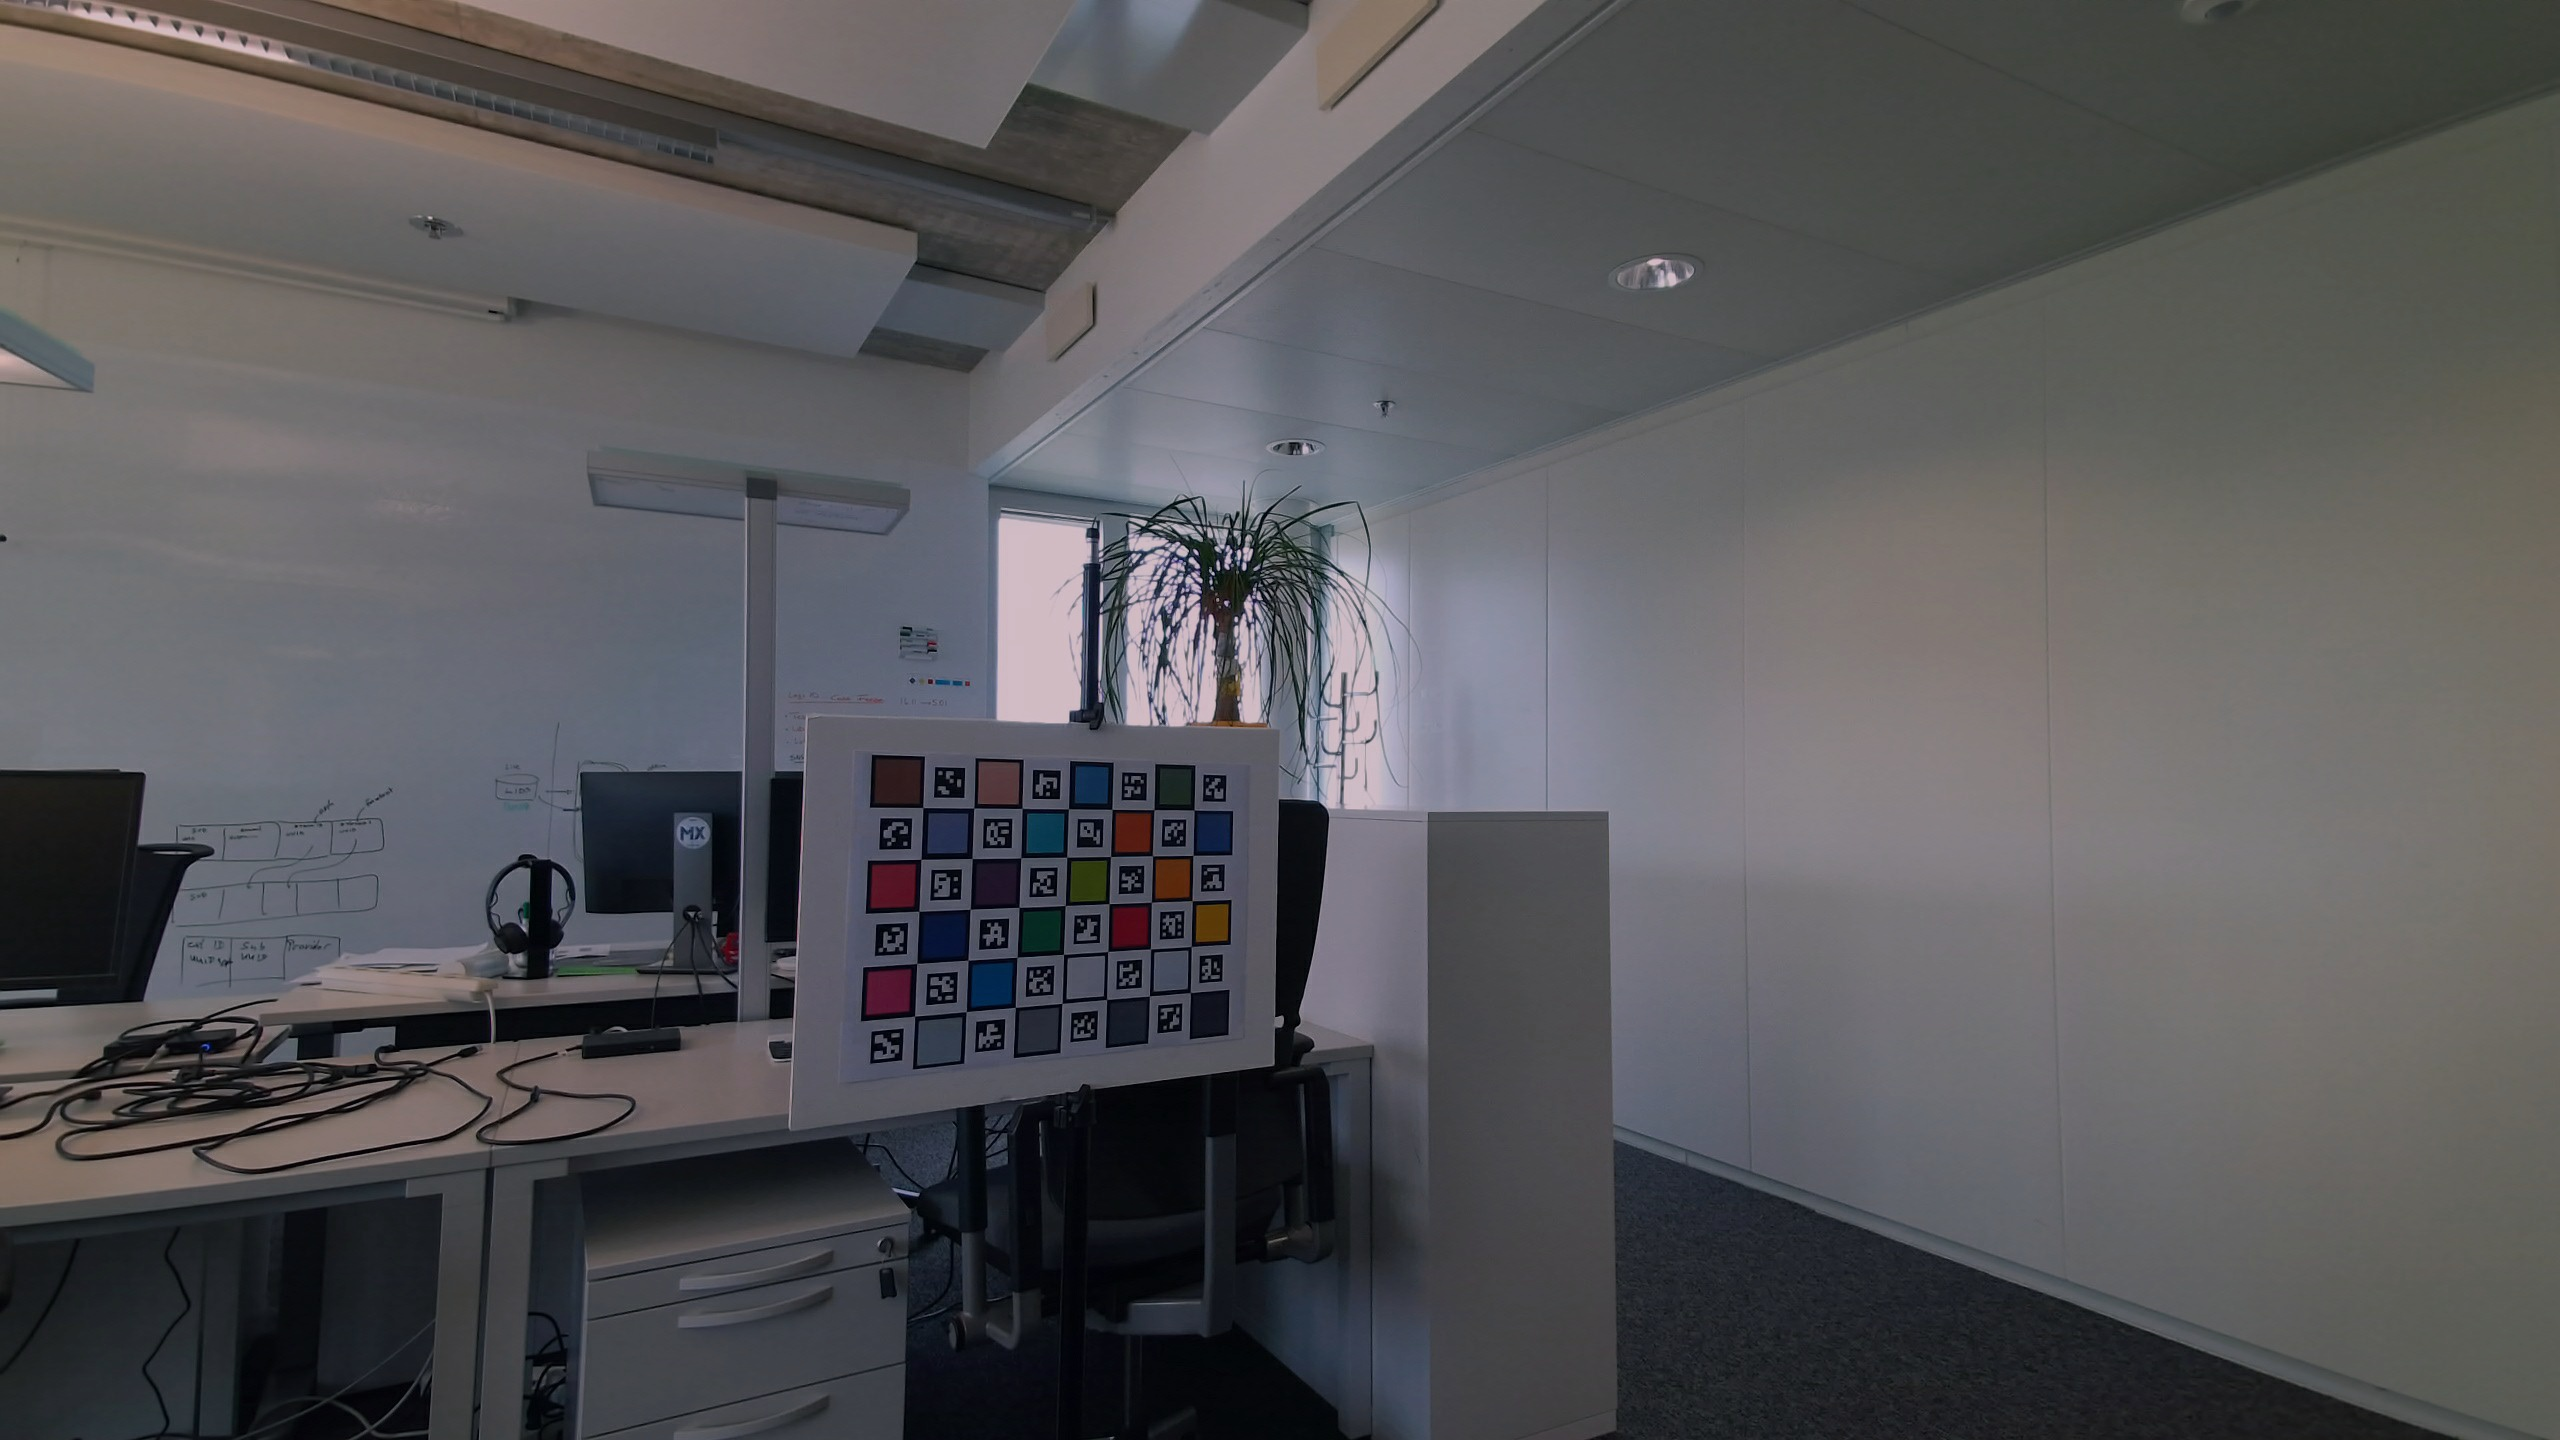
\includegraphics[width=0.50\textwidth]{images/visual_enhancement/colour/sub_poly_1_2015.jpg}
    \caption{Linear Least Squares Matching applied on the whole scene. The overall scene looks 'reddish' }
    \label{figure:sub_poly_1_2015}
\end{figure}


\textbf{RGB to RGB transform}

The RGB to RGB transform was found thanks to equation \ref{equation:rgbTOrgb}. It improves slightly colour consistency. However, the results weren't good enough to be used in the meeting room scenario.

\textbf{General Polynomial Transform}

As proposed in \cite{ilie_ensuring_2005}, a general polynomial transformed of the second order was calculated. Equation \ref{equation:general_polynomial_transform} was used to find the transform. The transformation decreases the colour differences for the 24 colours of the board. However, outside the colour squares, some artefacts appear. This approach gives bad results when applied to the whole scene.

\begin{figure}[H]
    \centering
    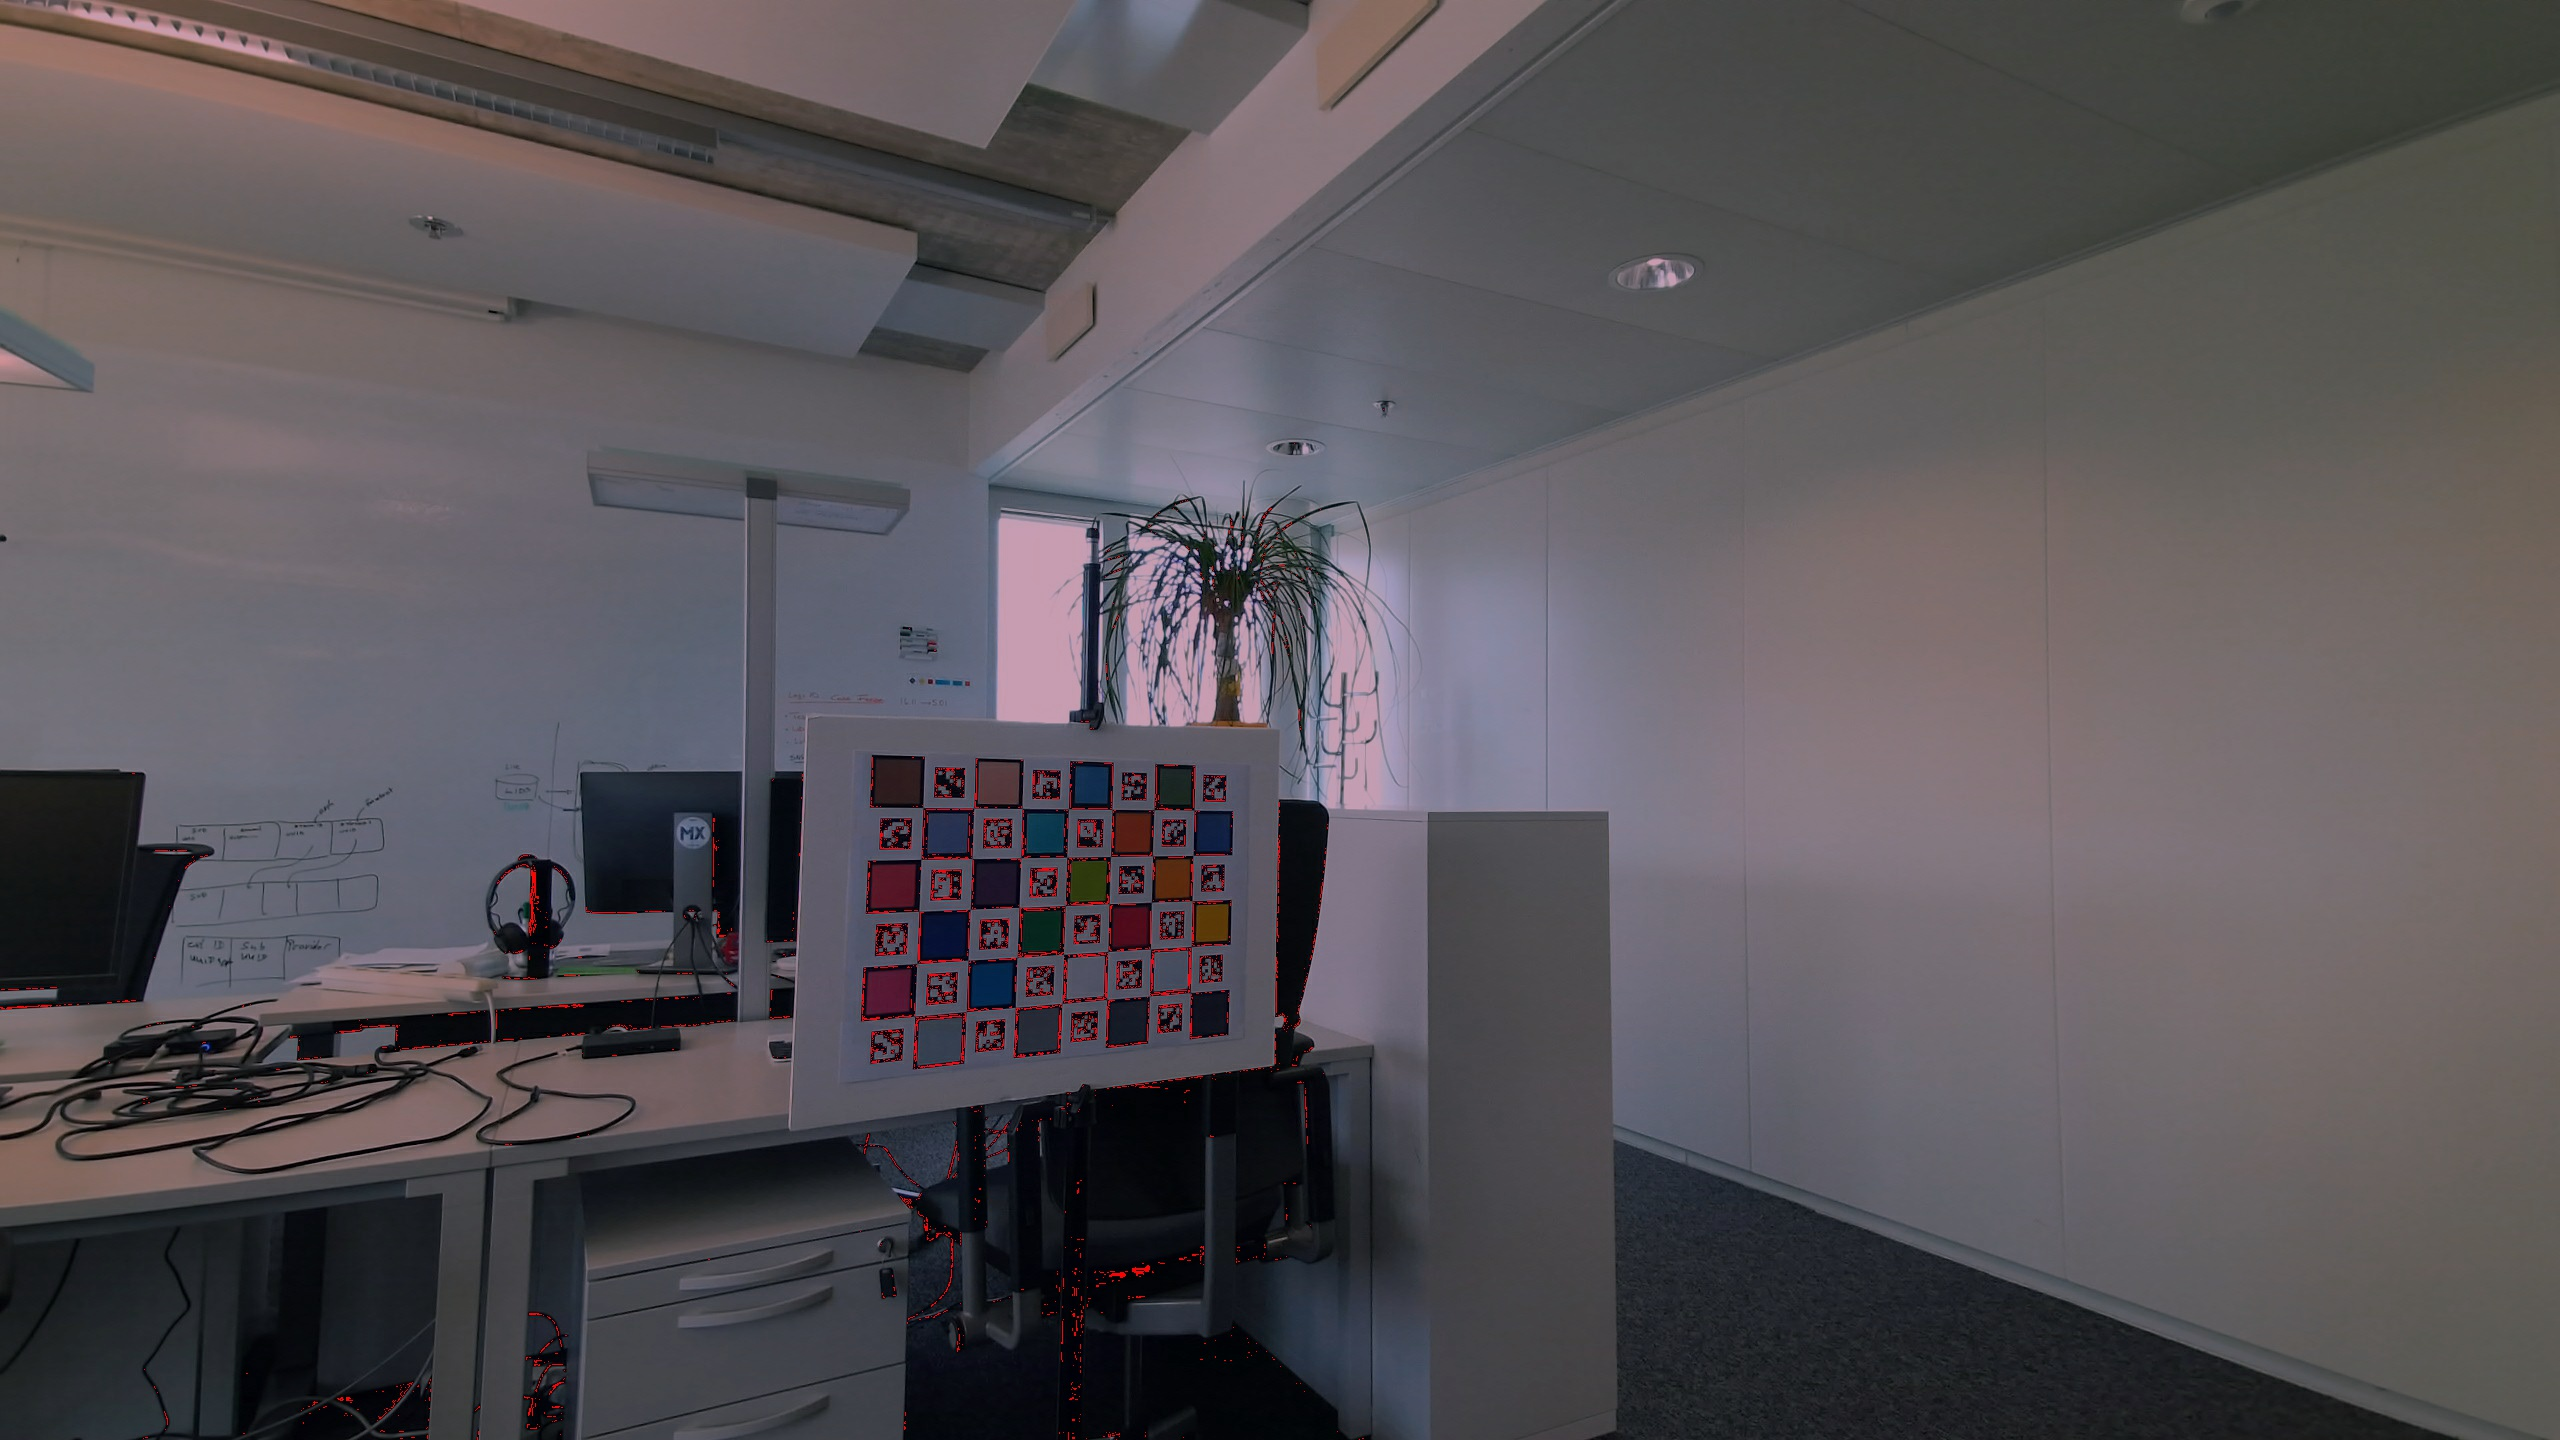
\includegraphics[width=0.50\textwidth]{images/visual_enhancement/colour/sub_poly_2.jpg}
    \caption{Second order polynomial transformation applied on the whole scene. Red artefacts are visible. The overall scene looks 'reddish' }
    \label{figure:sub_poly_2}
\end{figure}

\subsubsubsection{Colour Correction Using 3D Multiview Geometry}

The idea of \cite{eschbach_color_2015} was used on the same data coming from the colour checkerboard than in the experiment presented in the previous section \ref{section:exp_ens_checkerboard}. A fifth-order polynomial regression is proposed in \cite{eschbach_color_2015}. This transformation fit closely the 24 colours of the reference checkerboard. However, once applied to the whole scene, the output is full of artefacts, see figure \ref{figure:sub_poly_5_2015}.

\begin{figure}[H]
    \centering
    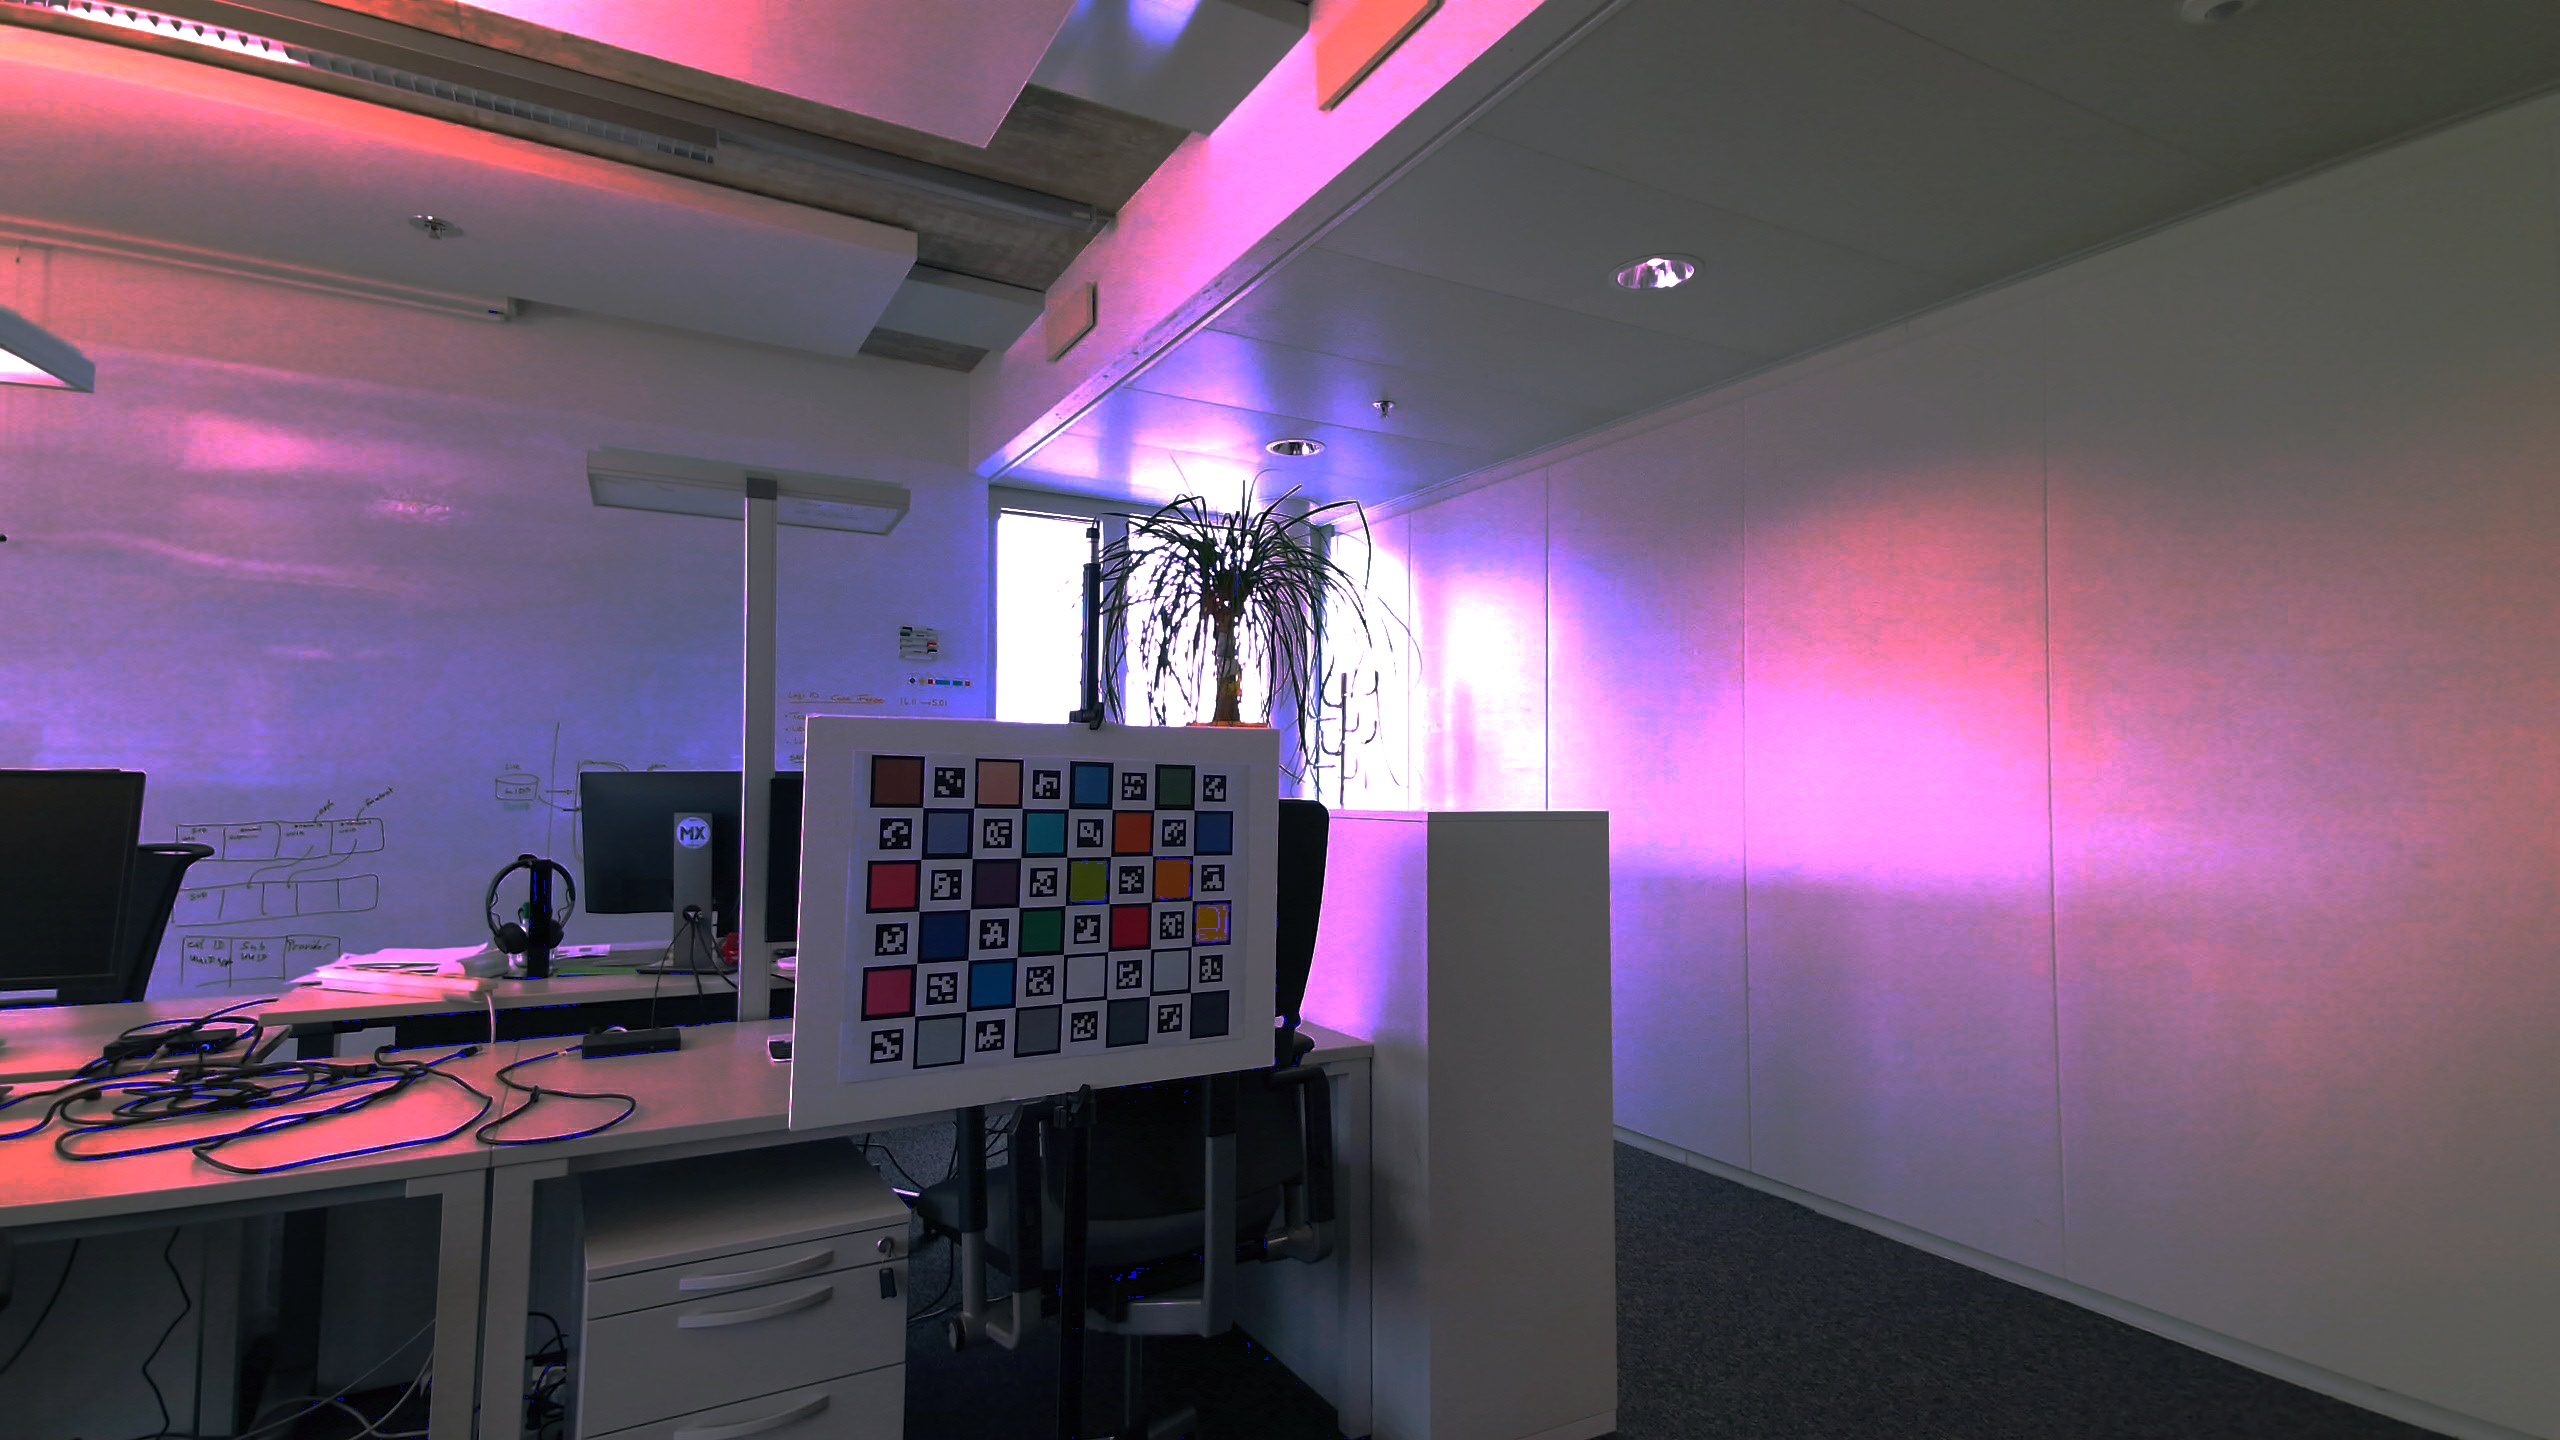
\includegraphics[width=0.50\textwidth]{images/visual_enhancement/colour/sub_poly_5_2015.jpg}
    \caption{Fifth order polynomial transformation applied on the whole scene. Red artefacts are visible. The overall scene looks 'reddish'}
    \label{figure:sub_poly_5_2015}
\end{figure}

Other order polynomial regressions were tried. They all have artefacts outside the colour squares of the checkerboard.

\subsection{Discussion}

The proposed method gives the best result for an application in a meeting room scenario. Focusing on the persons to correct the colour makes sense since they are the most interesting part of the scene. A correction based on the overlapping region makes sense if this region is relevant regarding the scene. Despite an improvement in the colour consistency, the result is not perfect. More advanced algorithms should be investigated.

The other algorithms tried gave less good results than the proposed one. The polynomial approach fits correctly the 24 colour given as target. Once it has to generalised to the whole scene, it fails. Artefacts appear and the output could be even worse than the original one. They were also tried in $Lab$ colour space. It wasn't concluding either. These approaches could suffer from the fact that it overfits the 24 colour in the target scene and therefore fails to generalise. Consequently they will not be used in the rendering pipeline.


Colour consistency across several cameras is a challenging and complex problem that could need a deeper analysis than the one done in this chapter. 